\chapter{Weibull analysis of partially observed lifetime data} \label{chap:chapter2}

Computerised maintenance management systems (CMMS) such as SAP \citep{sap} are now embedded in companies' maintenance policies and procedures, meaning that these companies now possess large datasets of component installation and replacement times. A natural use of these personalised failure time data sets is to tailor replacement strategies for the company's specific operating environments \citep[p. 13]{Meeker2022}, instead of solely relying on the manufacturer's recommendations. One problem, however, is that these large observational datasets collected through CMMS are much messier than the experimental ones used by manufacturers in traditional reliability/warranty analysis. This messiness comes about because of reporting issues, incomplete historical records, and the fact that most components are pre-emptively replaced before they fail because of the risk to production and employee safety. The result is that many of the valuable data sets stored in CMMS systems are incomplete because of censoring and left-truncation. On one hand, censoring occurs when the true lifetime of a failed component is not known, but either an upper bound, lower bound, or both are known. On the other hand, left-truncation arises when only units that have survived up until the point when failures begin being recorded are observable. The incomplete---censored and truncated---nature of such datasets means they are not strongly informative of the lifetime model.

The censored and left-truncated nature of such data makes what would otherwise be a very straightforward analysis far more complicated. Worse yet, the incompleteness of the data is not always obvious, and incorrect analysis can lead to biased results and misinformed decisions. The idler frame dataset introduced in Sec.~\ref{sec:industry-data} is one such case where data are both left-truncated and right-censored. Here, right-censoring arises due to the set of idlers in a frame either being preventatively replaced or still being in operation when the data were analysed; left-truncation arises since any idlers that were installed and failed before the time failures started being recorded in the CMMS are not present in the dataset but any that were installed before this time and failed after are. A further complicating factor of the idler frame dataset is that the installation times of idler frames that were already in operation when data started being captured in the CMMS are unknown, meaning that the left-truncated lifetimes are also censored and have unknown truncation times. This issue is sometimes referred to as unknown initial conditions or unknown exposure history \citep{guo1993}. Treatment of right-censored and left-truncated data was addressed by \citet{hong2009}, but not for cases with unknown exposure history of left-truncated samples. In this chapter, I propose a model for handling such cases in a Bayesian framework by imputing the unobserved portion of the left-truncated lifetimes with unknown exposure history and, along with them, the truncation times. I demonstrate the method using simulated data that mimics the observation process of the idler-frame data.

The incompleteness of a dataset that results from censoring and truncation reduces the information in the dataset, meaning that the data are only weakly informative of the model. In particular, when a large proportion of the dataset is right-censored, there is little information in the dataset about longer lifetimes---the upper tail of the lifetime distribution. To reduce uncertainty in the analysis of incomplete lifetime data, domain knowledge can be used to inform the model where the data cannot, but only if the prior is constructed properly. I show how to do this in the simulation example using an extension of an existing method for eliciting a joint prior for the parameters of a Weibull distribution \citep{kaminskiy2005}. I show how to properly implement the prior in a model for censored and truncated lifetime data and demonstrate how elicitation can be performed to encode information in different parts of the lifetime distribution. I then analyse the heavily censored and truncated simulated data using this extension.

In the next section, Sec.~\ref{sec:lifetime-data-background}, I provide a background of lifetime analysis, the Weibull distribution, and how censoring and truncation can be included in the likelihood. I then describe my proposed approach for modelling left-truncated data with unknown exposure history in Sec.~\ref{sec:lt-imputation}. The method imputes the unobserved portions of the left-truncated samples and their truncation times. The result of Sec.~\ref{sec:lt-imputation} is a likelihood that can account for data that is left-truncated with unknown exposure history and right-censored. The partial information in the data that this likelihood accounts for does not strongly inform the parameters. In such a case, using a weak or non-informative priors can, at best, leave areas of the posterior unusably diffuse and, at worst, place mass in spurious parts of parameter space. Therefore, in Sec.~\ref{sec:weibull-joint-prior}, I demonstrate how to construct an informative joint prior for the Weibull parameters. I introduce the method proposed by \citet{kaminskiy2005} for constructing the joint prior, point out its limitations, and describes my extensions of the method. In Sec.~\ref{sec:weibull-sim-example}, I demonstrate, using simulated data, my methods for imputing partially observed left-truncated lifetimes and encoding an informative joint prior. In this demonstration, I compare the imputation method alongside the case where we simply discard the partially observed left-truncated lifetimes and a case where we fully observe them (if we know their installation times). Sec.~\ref{sec:weibull-sim-study} presents a small simulation experiment where I repeat the simulation and model fitting in Sec.~\ref{sec:weibull-sim-example} for many different combinations of the simulation parameters to explore the limitations of the imputation approach. The chapter concludes with Sec.~\ref{sec:weibull-conclusion}, where I summarise the key contributions and findings from the chapter and provide recommendations for analysing lifetime datasets with right-censoring and left-truncated observations with unknown exposure histories, such as the idler-frame lifetime data. The recommendations distilled in this final section are applied to the idler-frame data in Chap.~\ref{chap:chapter3}. Table~\ref{tab:ch2-notation} provides a reference for the notation used in this chapter.

\begin{table}
    \centering
    \caption{\label{tab:ch2-notation}Nomenclature for the chapter.}
    \centering
    \begin{tabularx}{\textwidth}{lY}
    \toprule
    \cellcolor{gray!10}{$y$} & \cellcolor{gray!10}{The true value of a lifetime.}\\
    $\tilde{y}$ & The imputed value of a missing lifetime.\\
    \cellcolor{gray!10}{$y^O$} & \cellcolor{gray!10}{A lifetime that is fully observed; not left-truncated by the begining of observation or right-censored by the end.}\\
    $y^C$ & The true (unobservable) value of a lifetime that is censored at its end.\\
    \cellcolor{gray!10}{$y^T$} & \cellcolor{gray!10}{The value of a lifetime that is truncated at the beginning of its life.}\\
    $y^{TC}$ & The value of a lifetime that is truncated at the beginning of its life and censored at its end.\\
    \cellcolor{gray!10}{$c^{\textit{Lower}}$} & \cellcolor{gray!10}{The lower censoring time of a censored observation. If $c^{\text{Lower}} = 0$ the lifetime is left-censored.}\\
    $c^{\textit{Upper}}$ & The upper censoring time of a censored observation. If $c^{\text{Upper}} = \infty$ the lifetime is right-censored.\\
    \cellcolor{gray!10}{$c^{C;\textit{Lower}}$} & \cellcolor{gray!10}{The lower bound of a lifetime that is censored at the end of the lifetime.}\\
    $c^{TC;\textit{Lower}}$ & The lower bound of a lifetime that is censored at the end of the lifetime and truncated at the beginning.\\
    \cellcolor{gray!10}{$c^{T;\textit{Lower}}$} & \cellcolor{gray!10}{The lower bound of a lifetime that is truncated at the beginning of the lifetime when the exposure history is unknown.}\\
    $c^{T;\textit{Upper}}$ & The upper bound of a lifetime that is truncated at the beginning of the lifetime when the exposure history is unknown.\\
    \cellcolor{gray!10}{$\tau$} & \cellcolor{gray!10}{The left-truncation time.}\\
    $\tilde{\tau}$ & The imputed left-truncation time.\\
    \cellcolor{gray!10}{$\tau^{T}$} & \cellcolor{gray!10}{The left-truncation time of a lifetime truncated at its beginning but \textbf{not} censored at its end.}\\
    $\tau^{TC}$ & The left-truncation time of a lifetime truncated at its beginning \textbf{and} censored at its end.\\
    \cellcolor{gray!10}{$n^O$} & \cellcolor{gray!10}{The number of fully observed lifetimes; i.e. not truncated by the beginning of observation or right-censored by the end.}\\
    $n^C$ & The number of observations that are censored by the end of observation but not truncated by the beginning.\\
    \cellcolor{gray!10}{$n^T$} & \cellcolor{gray!10}{The number of observation that are truncated by the beginning of observations but not right-censored by its end.}\\
    $n^{TC}$ & The number of observations that are both truncated by the beginning of observation and right-censored by its end.\\

    \bottomrule
    \end{tabularx}
\end{table}
    

\section{Background} \label{sec:lifetime-data-background}

Lifetime analysis, also called survival analysis, is the analysis of failure time data from a population of particular components/assets to derive the risk of failure of a component depending on its level of exposure (usually some form of time) and sometimes other covariates \citep{moore2016}. From here on, I will use the general term unit/s to refer to individuals/groups of the same asset or component. Lifetime analysis of a population of units typically takes place by first specifying a sampling distribution for the lifetimes by choosing some parametric lifetime distribution for the units and incorporating any observational characteristics of the data, for example, censoring. Then, next, estimating the parameters of the distribution from failure time data using an appropriate inferential mechanism. Finally the fitted mode is used to derive useful reliability measures about the population which can inform asset management plans. When done in a Bayesian context, the first step of this process also includes specifying a prior distribution. From the resulting inference, we can devise replacement strategies that minimise the risk of unplanned replacements and, hence, the risk of lost production, as well as the cost of the maintenance strategy.

\subsection{Lifetime distribution}

The lifetimes of the units are modelled as a random variable $Y \in [0, \infty)$, the exposure time. $Y$ is some continuous or discrete exposure time from a clearly defined origin, the installation of the component, to a well-defined event, the component's failure. In reliability analysis, the exposure is typically absolute time, the operating time of the unit, or cycles of operation. For example, the idler-frame failures are recorded in absolute time since operating time is unavailable. Next, a specific parametric lifetime distribution is chosen for the random variable $Y$, $p(Y|\theta)$, and the parameters $\theta$ of the lifetime distribution are estimated from the data. Once the estimates are obtained, different properties of $Y$ can be used to draw useful insights in order to inform decisions \citep{hamada_2008}:
\begin{itemize}
    \item \textbf{Cumulative distribution function} (CDF), $F(y|\theta)$, is the probability that a unit will have failed by age $y$, i.e., $\text{Pr}\left[Y \le y|\theta\right]$. It is also sometimes called the cumulative risk function.
    \item \textbf{Survival function}, $S(y|\theta)$, is the complement of the CDF, i.e., $S(y|\theta) = \text{Pr}\left[Y > y|\theta\right] = 1 - F(y|\theta)$. It defines the probability of a unit surviving up to an exposure time $Y$. It is also sometimes called the reliability function ($R(y|\theta)$).
    \item \textbf{Hazard function}, $h(y|\theta)$, which is the instantaneous failure rate conditioned on the age of the unit. It can be calculated as $h(y|\theta) = p(y|\theta) / S(y|\theta)$.
\end{itemize}
For example, the CDF quantifies the risk of failures given a chosen preventative maintenance interval, and the hazard function identifies if a unit's risk of failure increases as it ages and, therefore, if a preventative maintenance strategy is even suitable at all.

\subsection{The Weibull distribution} \label{subsec:weibull-dist}

In the analysis that follows, I use the Weibull distribution to model the component lifetimes, that is
\begin{equation}
    Y|\beta, \eta \sim \hbox{Weibull}(\beta, \eta),
\end{equation}
where $\beta$ is the shape parameter and $\eta$ is the scale. The Weibull distribution is a commonly used lifetime distribution because of its ability to capture an increasing, constant, or decreasing risk of failure. In addition, the Weibull distribution is the limiting distribution for the minimum value in a sample when the sample space is lower bounded, such as lifetimes, which must be greater than zero. This characteristic of the Weibull distribution gives it a convenient interpretation in component reliability: the lifetime of a unit is the time of the first occurring catastrophic failure mode of the unit. In the analysis that follows, I use the coupled parameterization of the two-parameter Weibull distribution, which has PDF
\begin{equation}
    \label{eq:weibull-pdf}
    p_{W}(y|\beta, \eta) = \frac{\beta}{\eta}\left(\frac{y}{\eta}\right)^{\beta - 1} \exp^{-\left(\frac{y}{\eta}\right)^{\beta}},
\end{equation}
CDF
\begin{equation}
    \label{eq:weibull-cdf}
    F_{W}(y|\beta, \eta) = 1 - \exp^{-\left(\frac{y}{\eta}\right)^{\beta}},
\end{equation}
and hazard function
\begin{equation}
    h_{W}(y|\beta, \eta) = \frac{\beta}{\eta}\left(\frac{y}{\eta}\right)^{\beta - 1}.
\end{equation}
The shape parameter $\beta$ dictates whether the hazard increases $(\beta > 1)$, decreases $(\beta < 1)$, or stays constant $(\beta = 1)$. The effect of the shape parameter on the hazard function is demonstrated in Fig.~\ref{fig:hazard_function_demo}. Practically speaking, if the hazard function increases with exposure, this corresponds to a wear-out failure mechanism, whereas if it decreases, it corresponds to infant mortality. This distinction is important from a maintenance perspective because if the component does not wear out, a preventative replacement policy is not suitable \citep{jardine2013}. In other words, we want to be sure that $\beta > 1$ before implementing a preventative policy.

\begin{figure}[t]
    \centering
    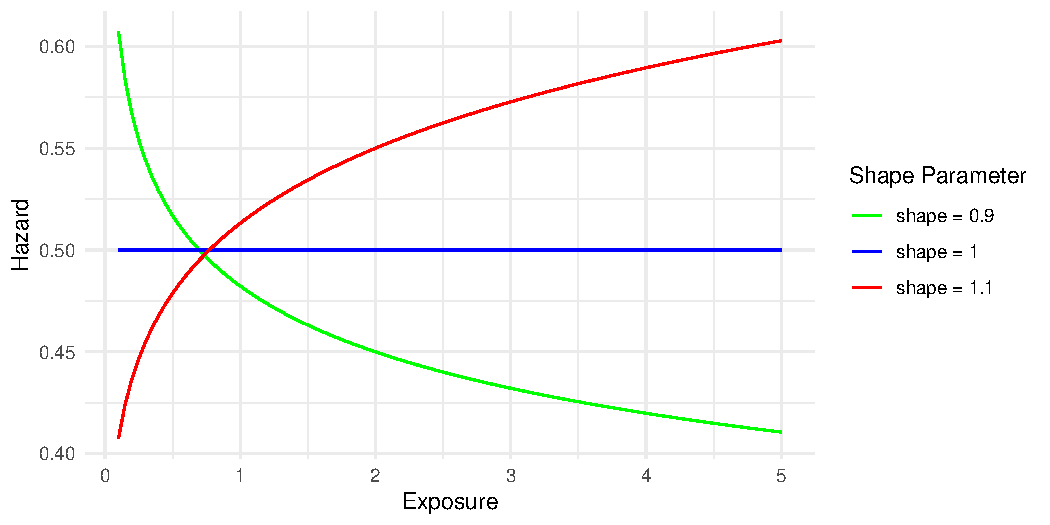
\includegraphics[width=1\textwidth]{./figures/ch-2/hazard_func_demo.pdf}
    \caption{The Weibull hazard function when $\beta = 0.9$, $\beta = 1$, or $\beta = 1.1$ and $\eta = 1$.}
    \label{fig:hazard_function_demo}
\end{figure}

\subsection{Censoring} \label{subsec:censoring-treatments}

It is very common for lifetime data to be censored \citep{tian2024}. Censoring occurs when we only partly observe the lifetime of a unit, or, in other words, we only observe upper and lower bounds for the lifetime. There are three types of censoring: left, interval, and right-censoring, but all three are treated in much the same way. Figure~\ref{fig:cense_examp} demonstrates these three types of censoring. For demonstration, say that you want to know the average lifetime of a light bulb to decide how many to buy for your house and Fig.~\ref{fig:cense_examp} shows an experiment with three bulbs. In the figure, the three bulbs are installed at time $t_0$, and you check if they are still operating at $t_1 = 0.5 \times 1000$ hours and again at $t_2 = 1 \times 1000$ hours. When you check at time $t_1$, one of the bulbs has failed and by the time you check again at $t_2$, so has another. Each unit's true, but unobserved, failure times are shown as crosses in the figure. The bulb that fails before $t_1$ is left-censored because you only observe an upper bound of the lifetime, and its true lifetime must be between $(0, t_1)$. The second bulb to fail is interval-censored since you observed it operating at $t_1$ but failed at $t_2$, and so its true value must be between the upper and lower bounds $(t_1, t_2)$. The third bulb, which has yet to fail, is right-censored since you only know that it has lasted longer than $t_2$ and, therefore, its true failure time must be in the interval $(t_2, \infty)$. Right and left-censoring are special cases of interval-censoring where the upper or lower bound of the lifetime is infinity or zero, respectively. Left-censoring is uncommon in reliability, so in the discussions that follow, I focus on right and interval-censoring. However, all of the methods presented in this chapter are easily extended to accommodate left-censored data.

\begin{figure}[h]
    \centering
    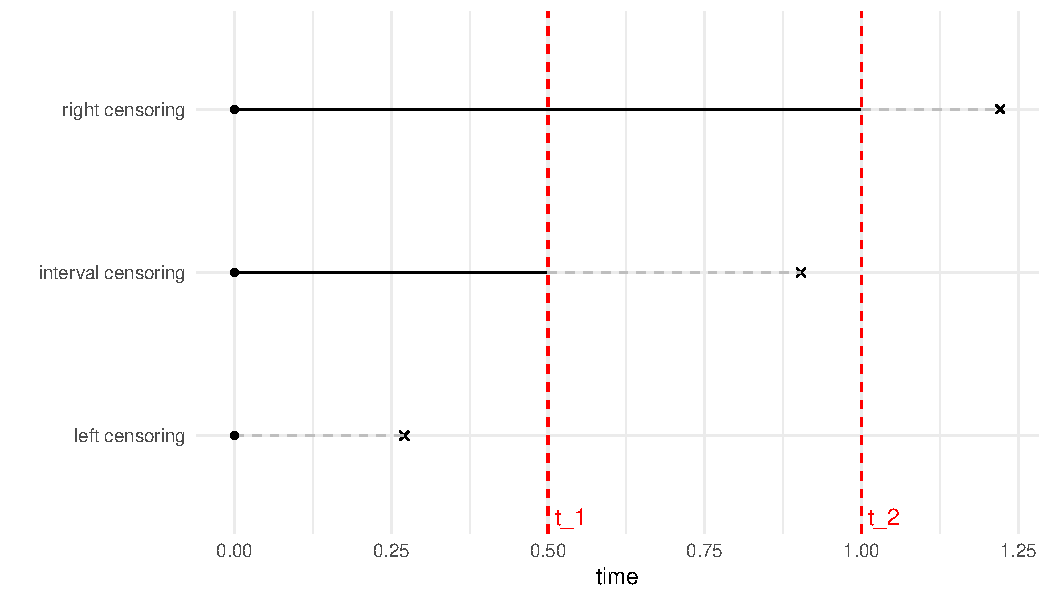
\includegraphics[width=1\textwidth]{./figures/ch-2/censoring_example.pdf}
    \caption{An example of the different types of censoring. Three units are installed at $t = 0$, indicated by a black dot, and their failure times are shown as black crosses. The units are inspected at times $t_1 = 0.5$ and $t_2 = 1$. The portion of the lifetimes that is observed is shown as a solid black line, and the unobserved (incomplete) portion is shown as a dashed grey line.}
    \label{fig:cense_examp}
\end{figure}

One way of handling censored data is to treat the censored lifetimes as missing data, which in a Bayesian framework is to treat them as a random variable (parameter) in the model \citep[p.211]{reich2019} and constrain their values to fall within the upper and lower censoring bounds \citep{stan_user_guide2024}\footnote{The Stan user guide shows how to impute censored observation in \href{https://mc-stan.org/docs/stan-users-guide/truncation-censoring.html}{\textit{Truncated or Censored Data}}.}. This is easily done during MCMC routines since, at each step, the imputed values can be sampled in the same way as the other parameters in the model. The distribution of the imputed censored lifetimes is assumed to have the same distribution as the rest of the population but constrained to be within the censoring bounds:
\begin{equation}
    \label{eq:impute-cens}
    \tilde{Y}^C_i|\beta, \eta \sim \hbox{Weibull}^{c^{\textit{\tiny{Upper}}}_i}_{c^{\textit{\tiny{Lower}}}_i}(\beta, \eta).
\end{equation}
Here $\tilde{Y}^C_i$ is the imputed value of the censored lifetime, and the superscript $c^{\textit{\tiny{Upper}}}$ and subscript $c^{\textit{\tiny{Lower}}}$ indicate that the distribution is constrained by the upper and lower censoring times. The imputed missing lifetimes are used to evaluate the full data likelihood in the same way as a typical lifetime dataset with no censoring. This approach of imputing the censored lifetimes is not unique to Bayesian methods. The same can be done using an Expectation Maximisation algorithm and maximum likelihood \citep{mitra2013}. However, using the Bayesian approach and MCMC methods, it is straightforward to derive uncertainty intervals for the parameters, imputed values, and useful quantities, which I show in Chap.~\ref{chap:chapter3}.

An alternative approach is to simply integrate out the censored observations as follows. The probability that a censored observation falls between the upper and lower censoring times is
\begin{align*}
    \label{eq:integrate-out-cens}
    \text{Pr}\left[c^{\textit{\tiny{Lower}}} < Y^C_i \leq c^{\textit{\tiny{Upper}}}\right] & = \int_{c^{\textit{\tiny{Lower}}}}^{c^{\textit{\tiny{Upper}}}} p_W\left(y^C_i\right) d y^C_i \\
    & = F_W\left(c^{\textit{\tiny{Upper}}}\right) - F_W\left(c^{\textit{\tiny{Upper}}}\right),
\end{align*}
where, as in eqs.~\eqref{eq:weibull-pdf} and~\eqref{eq:weibull-cdf}, $p_W(.)$ and $F_W(.)$ are the PDF and CDF of the Weibull distribution, respectively. By integrating out the censored observations, the likelihood can be written as
\begin{equation}
    \label{eq:censored_likelihood}
    L\left(\theta|\textbf{x}\right) = \prod^{n^O}_{i = 1}p_W(y^O_i)
    \prod^{n^C}_{j = 1}\left[F_W(c^{\textit{\tiny{Upper}}}_j) - F_W(c^{\textit{\tiny{Lower}}}_j)\right],
\end{equation}
where $\theta = \{\beta, \eta\}$ is the set of parameters of the Weibull lifetime distribution, $n^O$ and $n^C$ are the number of fully observed and censored observations, respectively, and $\textbf{x} = \{y^O_1, 
\dots, y^O_{n^O}, c^{\textit{\tiny{Upper}}}_1, \dots, c^{\textit{\tiny{Upper}}}_{n^C}, c^{\textit{\tiny{Lower}}}_1, \dots, c^{\textit{\tiny{Lower}}}_{n^C}\}$ contains the observed lifetimes and censoring times. This second approach is much more commonly used, particularly in the reliability literature (for example \citet{Meeker2022,tian2024,hong2009,mittman2013}). However, as I show later, it is convenient to frame the model using the first approach---where censored lifetimes are imputed---for the particular problem when data are also left-truncated with unknown installation times.

\subsection{Left-truncation}

Truncation arises when a sample comes from an incomplete population, in other words, there is some criterion that part of the population must satisfy in order to be observable \citep{guo1993}. Left-truncation, for example, arises when some units must survive up to a certain time to be observed. It is also possible for data to be right or doubly-truncated, but left-truncation is the most common in lifetime data, particularly in observational reliability datasets \citep{Emura2022}. The term `left-truncated observation' is often used to mean an observation that arises from a truncated population. The definition of left-truncation and left-censoring may seem very similar; however, they are distinctly different \citep{mitra2013}. Censoring is a characteristic of the sample, i.e., we know the number of left-censored observations but not the exact values of their lifetimes. In contrast, truncation is a characteristic of the population because we do not know how many lifetimes were not included in the dataset because those units did not survive past the truncation time, and hence, our sample is not representative of the true population. We can view censored units as known-unknowns and truncated units as unknown-unknowns. Left-truncated samples tend to over-represent longer lifetimes \citep{guo1993}. An example of a left-truncated dataset is shown in Fig.~\ref{fig:left_trunc_example}.

\begin{figure}[h]
    \centering
    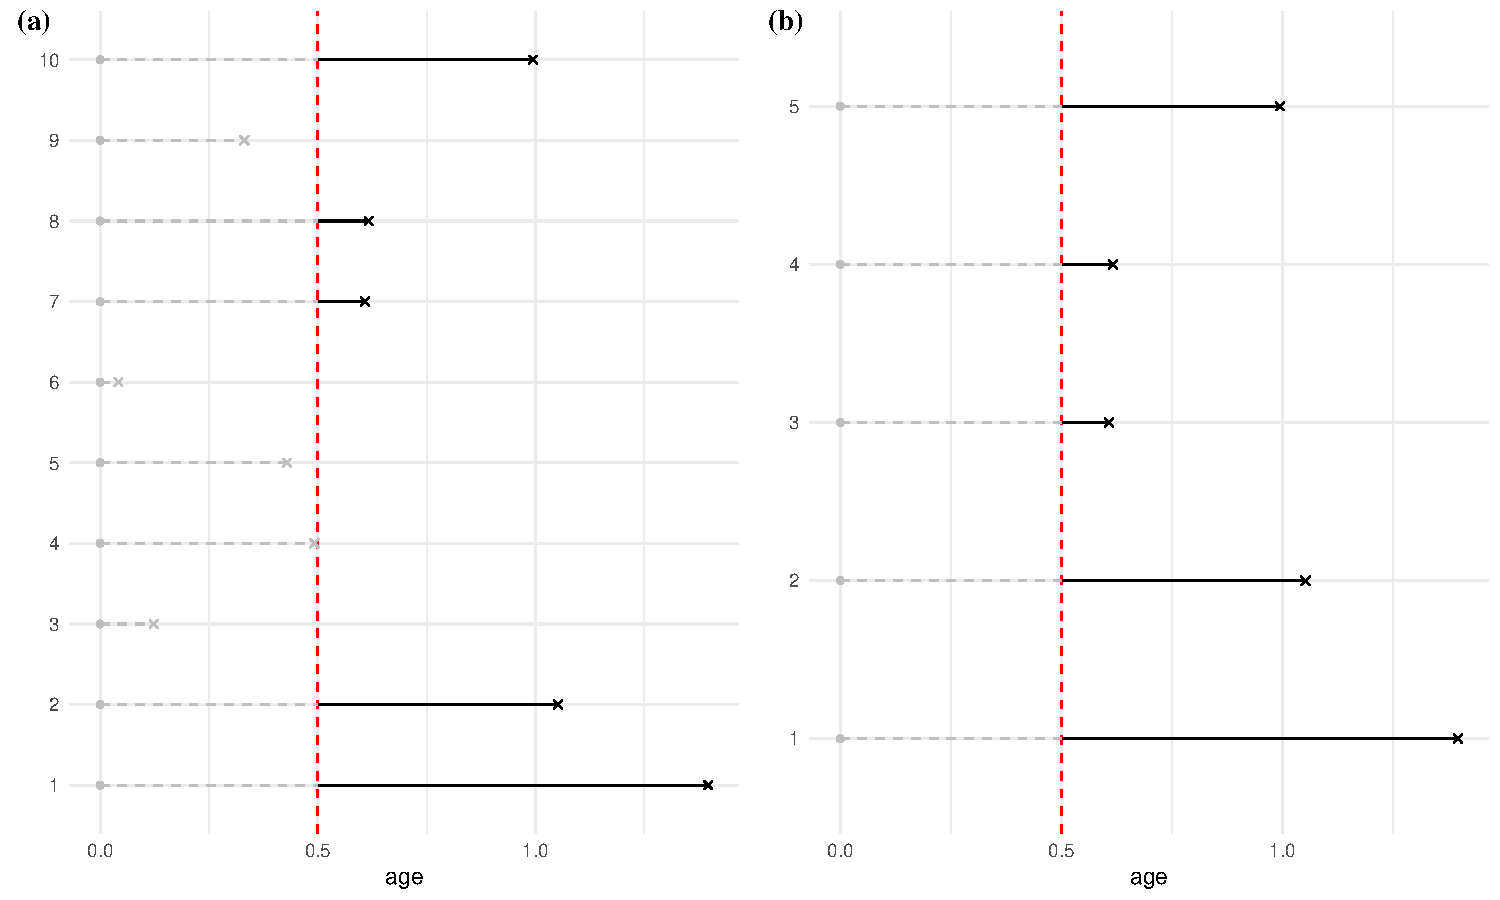
\includegraphics[width=1\textwidth]{./figures/ch-2/left_truncation_example.pdf}
    \caption{An example of the difference between (a) left-censoring in a dataset and (b) left-truncation. In (a), the lifetimes that fail before $t = 0.5$ are left-censored since their existence is known but not their exact failure time. In (b), any lifetimes that failed before the red line at $t = 0.5$ are absent from the dataset completely and therefore the likelihood of the observed data needs to be adjusted to reflect this.}
    \label{fig:left_trunc_example}
\end{figure}

Figure~\ref{fig:left_trunc_example} shows the difference between a data set with left-censoring and one that is left-truncated. Using the example of lightbulbs once again, consider that you test ten bulbs but only monitor their failures after $0.5 \times 1000$ hours. Figure~\ref{fig:left_trunc_example}~(a) shows a sample of ten lifetimes with the portion of lifetimes that sits to the left of the start of observation (the red line) greyed out to show that they are unobserved. In this case, lifetimes 2, 3, 4, and 8 are left-censored because you know that they were installed and that they failed sometime before $0.5 \times 1000$ hours. However, now imagine that someone else had tested the bulbs for $0.5 \times 1000$ hours and then gave you the six un-failed bulbs to perform your experiment (Fig.~\ref{fig:left_trunc_example}~(b)). In this case, you do not know that four bulbs have already failed, only that the bulbs you have are already $0.5 \times 1000$ hours old (the truncation time). Therefore, the probability of an observation that arises from a left-truncated distribution is $\text{Pr}\left[Y^T|Y^T > \tau^T\right]$ where $\tau^T$ is the truncation time. Therefore, the contribution of a left-truncated observation to the likelihood is
\begin{equation}
    \label{eq:left_trunc}
    L\left(\theta|y^T_i\right) = \frac{p_W\left(y^T_i\right)}{1 - F_W\left(\tau^{T}_i\right)},
\end{equation}
where the denominator re-normalized the density by the probability of surviving past $\tau^T$.

\subsection{Left-truncation and right-censoring} 

Observational reliability datasets commonly contain both left-truncated and right-censored observations. This combination naturally arises in observational datasets, such as those found in CMMS, where units are repeatedly replaced once they fail, and any units that were installed and failed before the start of the observation process (which might be the date a new CMMS was adopted) are absent in the dataset. Figure~\ref{fig:left_trunc_and_right_cens_example} shows a toy example, where three units are repeatedly replaced when they fail. We start to observe their failures at $t_{\text{start}}$ and stop at $t_{\text{end}}$. Any lifetimes that fail before $t_{\text{start}}$ are unobserved (greyed out in the figure), resulting in the first partialy observed lifetime of each unit being a left-truncated sample. Lifetimes that surpass $t_{\text{end}}$ are only partially observed (right-censored); hence, the portion of these lifetimes that sits to the right of $t_{\text{end}}$ is also greyed out in the figure. Returning to the example of light bulbs, say you recently moved into a new home and started recording the failures of bulbs in your home; the lifetimes of any bulbs that were already installed when you moved in would be left-truncated, and the lifetimes of any bulbs yet to fail are right-censored. \citet{hong2009}, \citet{mitra2013}, and \citet{kundu2016} analyse a dataset of electrical transformer failures that contains both left-truncation and right-censoring, and \citet{mittman2013} looks at a similar case for computer hard drives. The idler frame failure data that I analyse in Chap.~\ref{chap:chapter3} is also an example of this type of dataset since the idlers in the frames are repeatedly replaced when they fail. Replacement records of the idlers are only available from the end of 2014 onwards, but the conveyor has been in operation for much longer and is still in operation today.

\begin{figure}[h]
    \centering
    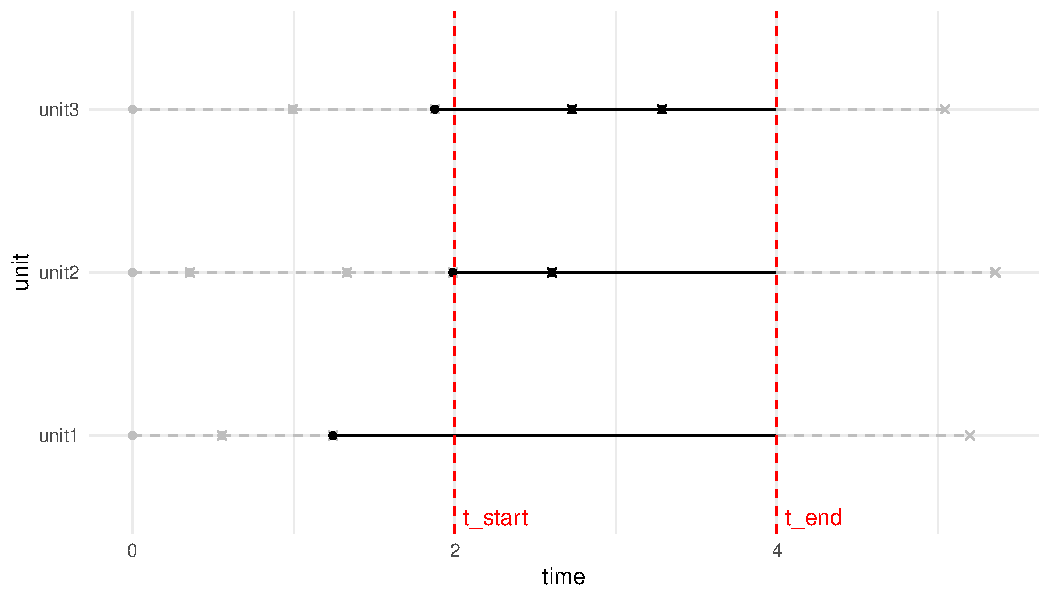
\includegraphics[width=1\textwidth]{./figures/ch-2/left_truncation_w_right_censoring_example.pdf}
    \caption{An example of how left-truncation and right-censoring arise from the repeated replacement of three units. Three units are shown on the vertical axis, and time on the horizontal. The failure times of the units are shown as black crosses, and every time a unit fails, it is instantaneously replaced. If we start observing these failures at $t_{start}$ and stop at $t_{end}$, then any lifetime that began before $t_{start}$ and failed after is left-truncated, and any lifetimes that began before $t_{end}$ and failed after are right-censored.}
    \label{fig:left_trunc_and_right_cens_example}
\end{figure}

\citet[eq.~(1)]{hong2009} shows that a likelihood for data that contain both left-truncated and right-censored can be written as,
\begin{align}
    \label{eq:left_trunc_and_right_cens_int}
    L\left(\theta|\hbox{\textbf{x}}\right) = & 
    \prod^{n^O}_{i = 1}\left[p_W(y^O_i) \right] \times
    \prod^{n^T}_{j = 1}\left[\frac{p_W(y^T_j)}{1 - F_W(\tau^T_j)} \right] \\
    & \times \prod^{n^C}_{k = 1}\left[1 - F_W(c^{C;\textit{\tiny{Lower}}}_k)\right]
    \times \prod^{n^{TC}}_{l = 1}\left[\frac{1 - F_W(c^{TC; \textit{\tiny{Lower}}}_l)}{1 - F_W(\tau^{TC}_l)}\right] \nonumber,
\end{align}
where the censored lifetimes are integrated out as in eq.~\eqref{eq:censored_likelihood}. The first term in eq.~\eqref{eq:left_trunc_and_right_cens_int} is the likelihood of the fully observed lifetimes; the second is the likelihood of a left-truncated observation given it has survived up until the truncation time; the third is the likelihood that the true age of a right-censored lifetime is greater than the censoring time; and the fourth is the likelihood that the true age of a left-truncated and right-censored lifetime is greater than the censoring time given that it survived past the truncation time. The symbols $n^O$, $n^T$, $n^C$, and $n^{TC}$ denote the number of fully observed lifetimes, left-truncated lifetimes, right-censored lifetimes, and lifetimes that are both left-truncated and right-censored, respectively. Following \citet{hong2009}, I write $\textbf{x} = \{y^O, y^T, \tau^T, c^{C;\textit{\tiny{Lower}}}, c^{TC;\textit{\tiny{Lower}}}, \tau^{TC}\}$ where $y^O = \{y^O_1, \dots, y^O_{n^O}\}$ is the set of fully observed lifetimes; $y^T = \{y^T_1, \dots, y^T_{n^T}\}$ the set of fully observed left-truncated lifetimes and $\tau^T = \{\tau^T_1, \dots, \tau^T_{n^T}\}$ their truncations times; $c^{C;\textit{\tiny{Lower}}} = \{c^{C;\textit{\tiny{Lower}}}_1, \dots, c^{C;\textit{\tiny{Lower}}}_{n^C}\}$ the set of right-censoring times of the right-censored observations; and $c^{TC;\textit{\tiny{Lower}}} = \{c^{TC;\textit{\tiny{Lower}}}_1, \dots, c^{TC;\textit{\tiny{Lower}}}_{n^{TC}}\}$ the set of right-censoring times of the lifetimes that are both right-censored and left-truncated and $\tau^{TC} = \{\tau^{TC}_1, \dots, \tau^{TC}_{n^{TC}}\}$ their truncation times. I note here that other publications, such as \citet{hong2009}, use indicator variables to identify if lifetimes are observed, right-censored, and/or left-truncated; however, I am explicitly splitting up the population because it makes it clear which lifetimes are observed and which are missing. \citet{kundu2016} also implement the same approach in a Bayesian framework using a Gibbs sampling algorithm to draw samples from the posterior.

\citet{mitra2013} takes the alternative approach of imputing the censored lifetimes using an Expectation Maximisation algorithm and the complete data likelihood, formulated as
\begin{align}
    \label{eq:left_trunc_and_right_cens_imp}
    L\left(\theta|\hbox{\textbf{x}}\right) = & 
    \prod^{n^O}_{i = 1}\left[p_W(y^O_i) \right] \times
    \prod^{n^T}_{j = 1}\left[\frac{p_W(y^T_i)}{1 - F_W(\tau^T_j)} \right] \\
    & \times \prod^{n^C}_{k = 1}\left[p_W(\tilde{y}^C_k)\right]
    \times \prod^{n^{TC}}_{l = 1}\left[\frac{p_W(\tilde{y}^{TC}_l)}{1 - F_W(\tau^{TC}_l)}\right] \nonumber,
\end{align}
where $\tilde{y}^C = \{\tilde{y}^C_1, \dots, \tilde{y}^C_{n^C}\}$ and $\tilde{y}^{TC} = \{\tilde{y}^{TC}_1, \dots, \tilde{y}^{TC}_{n^{TC}}\}$ are the imputed values of the censored and censored/truncated observations, and they are now included in the set of parameters $\theta = \{\beta, \eta, \tilde{y}^C, \tilde{y}^{TC}\}$. To simplify notation, I express the model in eq.~\eqref{eq:left_trunc_and_right_cens_imp} in a Bayesian framework as
\begin{align*}
    Y^O_i|\beta, \eta    & \sim \hbox{Weibull}(\beta, \eta) \\
    Y^T_j|\beta, \eta    & \sim \hbox{Weibull}(\beta, \eta) \qquad \qquad T[\tau^T_j, \;]\\
    \tilde{Y}^C_k|\beta, \eta    & \sim \hbox{Weibull}_{c^{C;\textit{\tiny{Lower}}}_k}(\beta, \eta) \\
    \tilde{Y}^{TC}_l|\beta, \eta & \sim \hbox{Weibull}_{c^{TC;\textit{\tiny{Lower}}}_l}(\beta, \eta) \quad T[\tau^{TC}_l, \;] \\
    \beta, \eta & \sim \pi(\theta_{\beta, \eta}),
\end{align*}
where the sequence of the first four expressions corresponds to the sequence of products of the likelihood in eq.~\eqref{eq:left_trunc_and_right_cens_imp}, $\hbox{Weibull}_{c^{\textit{\tiny{Lower}}}}$ indicates that the random variable has a Weibull distribution and is constrained to be greater than the right-censoring time, and $T[\tau, ]$ indicates that the distributions are re-normalised by the probability $\text{Pr}\left[Y > \tau\right]$ \citep{Stan2022} \footnote{This is the notation used in the Stan user manual in \href{https://mc-stan.org/docs/stan-users-guide/truncation-censoring.html}{\textit{Truncated or Censored Data}}.}. For the moment, I express the joint prior for the Weibull parameters in its most general form.

\paragraph{Unknown exposure history}

A problem arises when the installation time of the left-truncated lifetimes (lifetimes that begin before the start of observation) is unknown since, to re-normalise the truncated lifetime distribution of these observations, we must know how old they are at the beginning of observation $\tau^{\hbox{\tiny{T}}}$. For example, you probably would not know the ages of the lightbulbs in your house when you first moved in since you would not know when the previous owner installed them. The left-truncated observations in the idler frames dataset also have unknown exposure history since replacement records before 2014 are unreliable and not recorded at the frame level.

This problem is known as unknown exposure history or initial conditions \citep{guo1993}. In these cases, two approaches can be taken. The first is to discard all the left-truncated samples, in which case the parameter estimates are still unbiased. However, in doing so, we throw away a large amount of information. In most cases of left-truncation and right-censoring, the right-censoring masks any information about longer lifetimes, so the left-truncated samples are the only source of information about the upper tail of the lifetime distribution. The second approach is to assume a constant hazard, i.e. $\beta = 1$ since, in this case, the Weibull distribution reduces to the exponential and, no matter the age of a unit, the probability of it surviving a given period is constant (this is the memoryless trait of the exponential distribution). However, assuming a constant hazard is very restrictive and often, one of the aims of performing lifetime analysis in the first place is to determine if $\beta > 1$. Furthermore, assuming an exponential distribution when the data do not have a constant hazard may lead to severe bias in the parameter estimates \citep{heckman1986}. In Sec.~\ref{sec:lt-imputation}, I present a third option. I show how, by treating the unknown installation times as a case of censoring and imputing the censored data, the missing truncation times can also be imputed, and sensible parameter estimates can be obtained.

\section{Imputing unknown exposure histories} \label{sec:lt-imputation}

\paragraph*{Observed failure}
Using the toy example in Fig.~\ref{fig:left_trunc_and_right_cens_example}, say we do not observe any installation or failure times to the left of $t_\text{start}$. In this case, we know that each unit's first, partially observed lifetime started sometime between $t = 0$ and $t = t_\text{start}$. This is a case of interval-censoring, where the lower censoring bound $c^{T;\textit{\tiny{Lower}}}$ is the time from the beginning of observation to the failure time, and the upper bound is from $t = 0$ to the failure time $c^{T;\textit{\tiny{Upper}}}$.

In many practical applications, there will be no clear origin $t = 0$ with which to calculate an upper bound for an interval-censored lifetime, and the analyst will need to make an informed decision. For example, in the light bulb example, $t = 0$ may be when the house was first built or when the particular type of bulb started being manufactured, whichever is more recent. For the case of the idler-frames, $t = 0$ is the date that the conveyor was first commissioned. If there is no sensible choice of $t = 0$, then the lifetimes with unknown exposure histories could be treated as right-censored, in which case $c^{T;\textit{\tiny{Upper}}} = \infty$, but the following method could still be applied. In this case, the right-censoring time is relative to the end of the lifetime, rather than the beginning, like typical right-censored observations.

Treating the left-truncated lifetimes with unknown exposure history as interval-censored, their distribution is
\begin{equation}
    Y^T_j|\beta, \eta \sim \hbox{Weibull}^{c^{T;\textit{\tiny{Upper}}}_{j}}_{c^{T;\textit{\tiny{Lower}}}_{j}}(\beta, \eta) \quad T[\tilde{\tau}^{T}_j, \;],
\end{equation}
where the missing truncation time $\tilde{\tau}^{T}_j$, needed to renormalise the contribution to the likelihood, is calculated from the imputed value of the lifetime as
\begin{equation}
    \label{eq:missing-trunc-time}
   \tilde{\tau}^T_i = \tilde{y}^T_i - c^{T;\textit{\tiny{Lower}}}_{j}.
\end{equation}

In the lightbulb example, say you moved into a house a year ago and the previous owner had built the house five years before. Any lightbulbs that was installed when you moved in and failed within the year that you have been living there are left-truncated lifetime with unknown exposure history. For instance, say a bulb that was installed when you moved in failed after six months. Using the imputation method, you impute the lifetime of this bulb, which you know should be between six months and five years and six months. For example, if the imputed age is four years, according to eq.~\eqref{eq:missing-trunc-time}, the imputed truncation time would be three years and six months: the imputed value of the lifetime minus the time you have observed it for.

\paragraph*{Censored failure}
When the lifetime is both interval-censored by the start of the observation period and right-censored by the end, such as unit 1 in Fig.~\ref{fig:left_trunc_and_right_cens_example}, it is not possible to calculate the missing truncation time according to eq.~\eqref{eq:missing-trunc-time}. For example, consider a light bulb that was installed when you moved into your house and is still operating after the one year that you have lived there. The value of such a lifetime can be imputed, like any right-censored observation, from the distribution
\begin{equation}
    \tilde{Y}^{TC}_l|\beta, \eta \sim \hbox{Weibull}_{c^{TC;\textit{\tiny{Lower}}}_{l}}(\beta, \eta) \quad T[\tilde{\tau}^{TC}_l, \;], 
\end{equation}
where the censoring time is the period that you observed its operation $c^{TC;\textit{\tiny{Lower}}} = t_{end} - t_{start}$. This is the same as right-censoring because for a bulb that was installed when you moved in and is yet to fail, you only know that the lifetime is longer than the one year you have lived in the house, which is right-censoring. However, because there is no observed installation or failure time, $\tilde{\tau}^{TC}$ can take on any value between zero and $\min\left(t_\text{start}, \tilde{y}^{TC}_i - c^{TC;\textit{\tiny{Lower}}}\right)$. I impute the truncation time from
\begin{equation}
    \label{eq:imp-trun-times}
    \tau^{TC}_l \sim \hbox{Unif}\left(0, \min\left(t_\text{start}, \tilde{y}^{TC}_l - c^{TC;\textit{\tiny{Lower}}}_l\right)\right),
\end{equation}
where $c^{TC;\textit{\tiny{Lower}}}$ is the right-censoring time, in other words, the time that we observed the lifetime for. Sampling the value of $\tilde{\tau}^{TC}$ in this way will incorporate the uncertainty around the installation times of these lifetimes in the posterior. For example, for a light bulb that has been in operation the entire time that you have lived in your house (one year) you impute a value for the missing value. If the imputed value is two years, then the missing truncation time could be anywhere from zero (if the bulb was installed just before you moved in) to one year (if the bulb fails immediately after you perform your analysis). However, if the imputed value is seven years, then the truncation period can only be between zero and five years because the bulb could not have been installed before the house was built.

The method to impute the missing lifetimes and left-truncation times of the left-truncated lifetimes with unknown exposure history allows the information in the these incomplete observations to be retained in the analysis. However, incomplete data such as these lifetimes and the right-censored ones are typically only weakly informative of the parameters \citep{tian2024}. When this is the case, the model for the data should be paired with a well constructed informative prior that ensures that the posterior does not have mass in implausible ares of parameter space. 

\section{Informative joint prior} \label{sec:weibull-joint-prior}

In cases where data only provide partial information, such as lifetime data where some lifetimes are masked by censoring, an informative prior can help to `fill in the gaps' and inform areas of the lifetime distribution that the incomplete data cannot. For example, right-censoring masks the upper tail of the lifetime distribution, and if there are no observed failures beyond some censoring time, then the data do not contain any information that informs this upper tail. This will become clear in Sec.~\ref{subsec:weibull-model-fits} when I fit a Weibull distribution to censored lifetimes after discarding any truncated lifetimes. An added motivation for using an informative prior in these cases is that non-informative priors can place mass in implausible parts of the parameter space, and when combined with a weak likelihood, where the data are not strongly informative of the parameters either due to small a sample size, incomepleteness, or identifiability issues, this can leads to spurious parameter estimates \citep{tian2024}.

\citet{kaminskiy2005} proposed a method for encoding an informative joint prior for the two parameters of the Weibull distribution by eliciting information about cross sections of the Weibull CDF. In their method, the analyst provides an informed estimate of the expected value of the CDF at two exposure times, $t_1$ and $t_2$, and the level of uncertainty around these estimates. The pair of estimate and uncertainty level at each exposure time $(\mu_{\hat{F}_{t_i}}, \sigma_{\hat{F}_{t_i}})$, $i = \{1, 2\}$, are encoded as the mean and standard deviation of a beta distribution. Then, by sampling realisations of the CDF at each exposure time $(\hat{F}_{t_1}, \hat{F}_{t_2})$ from the two beta distributions, ensuring that $\hat{F}_{t_1} < \hat{F}_{t_2}$, the parameters of the Weibull CDF that passes through the two realisations can be calculated to obtain a draw from the informative joint prior. \citet{kaminskiy2005} then show how to obtain a Bayesian point estimate of the CDF at some new exposure time $t_3$ where binomial failure data are available. To do so, they calculate the parameters of a new beta distribution that describes the CDF at $t_3$ according to the joint prior draws, and then update the parameter estimates of the beta distribution at $t_3$ with the data, taking advantage of the beta-binomial conjugacy.

The method for obtaining joint draws from an informative prior for the two Weibull parameters is consistent with the recommendations of \citet{gelman_workflow_2020}, who suggest eliciting information on the outcome space---which is more familiar to domain experts---and then translating this information into an informative prior in the parameter space that also indirectly describes how the parameters should be allowed to covary with one another. An alternative method proposed by \citet{Meeker2022} is to reparameterise the distribution in terms of the shape $\beta$ and some quantile, $q_r$, of the distribution and then specify independent priors for $\beta$ and $q_r$. Both methods have proven useful in practice and have been implemented in reliability software \citep{krivtsov2017}. However, it can be difficult for practitioners unfamiliar with Weibull analysis to elicit information about $\beta$. Therefore, I develop a variation of \citeauthor{kaminskiy2005}'s method for obtaining draws from a joint informative prior for the Weibull parameters. I build upon their method by elaborating on what it means to elicit information at different values of $t_1$ and $t_2$ and how this translates into covariance in the joint distribution. I implement the joint prior in a lifetime model so that the draws from the prior are properly filtered through the likelihood.

The method of \citet{kaminskiy2005} provides only point estimates of the updated parameter values of the beta distribution at $t_3$. To obtain corresponding values of the Weibull parameters, the analyst must once again sample pairs of realisations along the CDF---now at either $t_3$ and $t_1$ or $t_3$ and $t_2$---and calculate the parameters of the Weibull CDF that passes through the two points. In doing so, he/she `reuses' the prior distribution at either $t_1$ or $t_2$ to generate the posterior, and so the `prior belief' about the CDF at whichever time is used is not updated. Furthermore, the resulting joint draws will be sensitive to whether $t_1$ or $t_2$ is used to generate the joint posterior distribution of the Weibull parameters. By instead implementing the method for obtaining draws from the joint prior within the HMC sampling algorithm, I show how to properly filter the prior through the likelihood to obtain the full posterior. Doing so also means that the prior can be updated with lifetime data (i.e., failure times rather than binomial trial data), censoring and truncation information can be included in the likelihood, and consequently a proper Bayesian joint posterior is obtained for the two Weibull parameters. 

Instead of beta distributions, I use normal distribution truncated between zero and one to encode prior belief about the CDF at $t_1$ and $t_2$. When specifying prior information close to the upper and lower tails of the Weibull CDF a beta distribution places a lot of mass very close to zero or one, which can cause numerical issues during sampling. Truncated normal distributions are much better behaved. The prior can therefore be expressed as
\begin{align*}
    \hat{F}_{t_1} \sim & \hbox{N}^{1}_{0}(\mu_{\hat{F}_{t_1}}, \sigma_{\hat{F}_{t_1}})             \\
    \hat{F}_{t_2} \sim & \hbox{N}^{1}_{\hat{F}_{t_1}}\left(\mu_{\hat{F}_{t_2}}, \sigma_{\hat{F}_{t_2}}\right) \\
    \beta            = & \frac{g(\hat{F}_{t_2}) - g(\hat{F}_{t_1})}{\log(t_1 / t_2)}               \\
    \eta             = & \exp\left[\log(t_1) - \frac{\hat{F}_{t_1}}{\beta}\right]
\end{align*}
where $g(\hat{F}) = \log(-\log(1 - \hat{F}))$ and the superscript and subscripts on the normal distribution indicate the upper and lower constraints of the support.

Depending on the choice of $t_1$ and $t_2$, the analyst encodes different information into the joint prior, which is reflected in how the two parameters covary with one another. For demonstration, plots (a), (b), and (c) in Fig.~\ref{fig:kaminskiy-join-priors} show the draws from three different joint priors constructed using this elicitation method. To construct the prior, I specify some `true' values of the parameters $(\beta = 1.1; \eta = 1)$ and then specify the priors to reflect the true value of the CDF at different quantiles $t_i = q_r$, where $r$ specifies the probability, so that all of the priors contain the `true' parameter values. Figure~\ref{fig:kaminskiy-join-priors}~(a) shows a prior where information is encoded at early exposure times ($t_1 = q_{0.05}$ and $t_2 = q_{0.20}$), (b) shows one where information is encoded around the median age ($t_1 = q_{0.40}$ and $t_2 = q_{0.60}$), and (c) shows one where the elicitation times are in the upper tail of the lifetime distribution($t_1 = q_{0.90}$ and $t_2 = q_{0.99}$). Plots (d), (e), and (f) in Fig.~\ref{fig:kaminskiy-join-priors} show the corresponding uncertainty around the Weibull CDF that results from the different priors in (a), (b), and (c), respectively. We see that the joint prior allows us to express our prior belief in one area of the PDF while allowing the prior to be vague in others. This characteristic has useful application in the context of heavy censoring since censoring masks longer lifetimes and hence increases uncertainty in the upper tail of the distribution but still contains useful information in the lower tail.

\begin{figure}
    \centering
    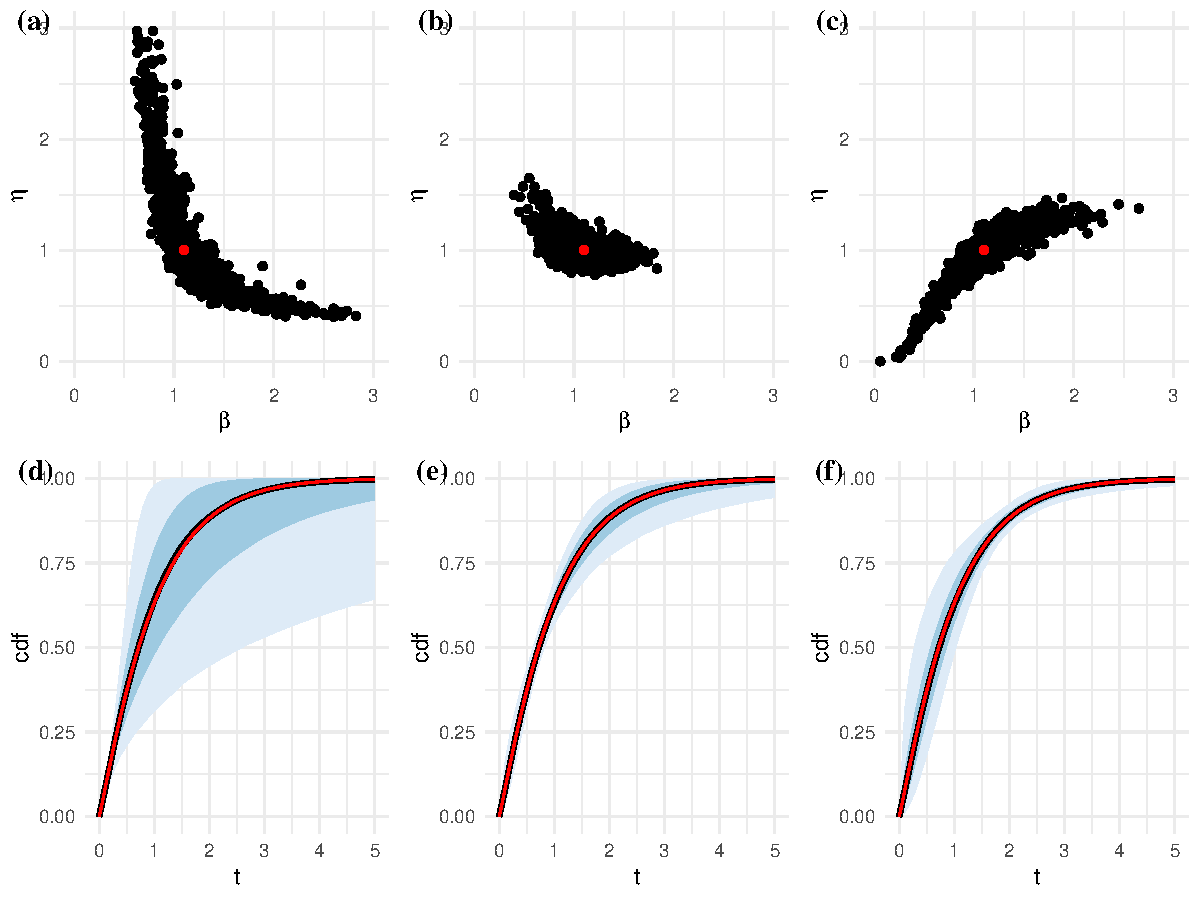
\includegraphics[width=1\textwidth]{./figures/ch-2/joint-priors.pdf}
    \caption{Three different informative joint priors constructed using the adaptation of the method of \citet{kaminskiy2005}. The joint draws of the parameters are shown in the top row---(a), (b), and (c)---and the corresponding uncertainty in the CDF is shown in the bottom---(d), (e), and (f). (a) and (d) show a prior where information is elicited around $t_1 = 0.07$ and $t_2 = 0.26$ (the 0.05 and 0.20 quantiles of the true distribution $\hbox{Weibull}(1.1, 1)$), (b) and (e) show a prior where information is elicited around $t_1 = 0.46$ and $t_2 = 1.04$ (the 0.35 and 0.65 quantiles), and (c) and (f) show a prior elicited at $t_1 = 1.54$ and $t_2 = 2.71$ (the 0.80 and 0.95 quantiles).}
    \label{fig:kaminskiy-join-priors}
\end{figure}

In Sections~\ref{sec:weibull-sim-example} and~\ref{sec:weibull-sim-study}, I compare the informative joint prior shown in Fig.~\ref{fig:kaminskiy-join-priors}~(c) and~(f), which encodes information in the upper tail, with the vague independent priors $\beta \sim \hbox{N}^{+}(1.1, 1)$ and $\eta \sim \hbox{N}^{+}(1, 1)$, where the superscript $(+)$ indicates that the prior is truncated to be positive. 

\section{Analysis of simulated data} \label{sec:weibull-sim-example}

In this section, I demonstrate the proposed method for imputing the left-truncated samples with unknown exposure time using data simulated in a way that emulates the idler-frame observation process. Repeated replacements of a set of units are simulated from a $\hbox{Weibull}(1.1, 1)$ distribution and left-truncation and right-censoring produced in the simulated dataset by only retaining the failures that occur within an observation period. I then fit a Bayesian model, which imputes any partially observed lifetimes in the dataset, and compare the results with two alternative analyses: one where the left-truncated samples are discarded, and only the fully observed and right-censored observation are used to estimate the Weibull distribution, and another where the left-truncated lifetimes are fully observed. The latter is the ideal scenario, since if the left-truncated lifetimes are fully observed then the likelihoods in either eq.~\eqref{eq:left_trunc_and_right_cens_int} or~\eqref{eq:left_trunc_and_right_cens_imp} can be used to model the data. I compare the three different cases using both vague independent priors for the Weibull parameters and an informative joint prior. The six model-prior treatment combinations of the simulated data are laid out in Table~\ref{tab:model-prior-comb}. 

The simulation experiments in this section show that, for small samples, the imputation approach gives almost the same inference as the case where we know the true installation times. When we throw out all of the left-truncated observations, there is a large increase in uncertainty, particularly around the upper tail of the lifetime distribution. However, if an informative joint prior is carefully constructed to inform the upper part of the distribution, then the results of the three different analyses are very similar. In Sec.~\ref{subsec:sim-method-weibull}, I explain how I simulate data that emulates the data-generating process of the idler-frames. I then analyse the simulated data in Sec.~\ref{subsec:weibull-model-fits} using the three different approaches and a vague prior and compare the posteriors. In Sec.~\ref{subsec:weibull-model-fits-informative}, I repeat the three analyses using an informative joint prior and compare the posterior distributions again.

\begin{table}
    \centering
    \begin{multicols}{2}
    
    \textbf{Model treatments}
    \begin{itemize}
        \item[] \emph{Including left-truncation}\\ The samples that are left-truncated by the beginning of observation have known exposure history and are fully accounted for using the likelihood in eq.~\eqref{eq:left_trunc_and_right_cens_int} or~\eqref{eq:left_trunc_and_right_cens_imp}.
        \item[] \emph{Discarding left-truncation}\\ The samples that are left-truncated by the beginning of observation have unknown exposure history and are discarded, leaving only the fully observed and right-censored lifetime data to estimate the lifetime distribution \citep{guo1993}.
        \item[] \emph{Imputing left-truncation}\\ The samples that are left-truncated by the beginning of observation have unknown exposure history and the method proposed in Sec.~\ref{sec:lt-imputation} is used to impute their true values and truncation times.
    \end{itemize}

    \columnbreak
    
    \textbf{Prior treatments}
    \begin{itemize}
        \item[] \emph{Weakly informative}\\ Normal distributions that place mass over a wide but plausible range of parameter space:
        \begin{align*}
            \beta \sim & \hbox{N}^{+}\left(1.1, 1\right)  \\
            \eta \sim & \hbox{N}^{+}\left(1, 1\right).
        \end{align*}
        \item[] \emph{Strongly informative}\\ A well constructed prior that encodes information about the CDF at $t_1 = 1.54$ and $t_2 = 2.71$ to encode information about the upper tail of the lifetime distribution:
        \begin{align*}
            \hat{F}_{t_1} \sim & \hbox{N}^{1}_{0}\left(0.8, 0.1\right)    \\
            \hat{F}_{t_2} \sim & \hbox{N}^{1}_{\hat{F}_{t_1}}\left(0.95, 0.05\right).
        \end{align*}
    \end{itemize}

    \end{multicols}
    \caption{The different model-prior combinations fitted to the simulated data.}\label{tab:model-prior-comb}
\end{table}

\subsection{Simulation method} \label{subsec:sim-method-weibull}

To simulate data that emulates the idler-frame lifetime data set, I
\begin{enumerate}
    \item Sample $N \times M$ draws from a Weibull distribution with known shape parameter $\beta = 1.1$ and scale parameter $\eta = 1$ (where $M$ is the number of units and $N$ is chosen to be sufficiently large so that the repeated replacement process surpasses the end of the observation period).
    \item Assign these lifetimes to $M = 10$ units.
    \item Calculate failure times rather than lifetimes, by taking the cumulative sum of the $N$ lifetimes assigned to each unit. The installation times are calculated by taking the lag of the failure times.
    \item Define a start, $t_{start} = 5$, and end time, $t_{end} = 6$, for the observation window, and discard any lifetimes where both the install and failure times sit either before $t_{start}$ or after $t_{end}$.
    \item Mark the remaining lifetimes as left-truncated and/or right-censored if the install time is less than $t_{start}$ or if the failure time is greater than $t_{end}$, respectively. If a lifetime is left-truncated, then I set $t_{start}$ as the observed start of the lifetime and if a lifetime is right-censored, I substituted $t_{end}$ as the observed failure time.
\end{enumerate}
Table~\ref{tab:sim-cmms-data} presents a dataset simulated using the method in steps 1--5 above. The simulated observations are also plotted in Fig.~\ref{fig:sim_censored_units}, where the start and end of observation are shown as red vertical lines, and the observed portions of the simulated data are shown in black and the unobserved `incomplete' part is shown in grey. Note that if we were to throw away the left-truncated samples, then we would be discarding more than 50\% of the sample.

\begin{figure}
    \centering
    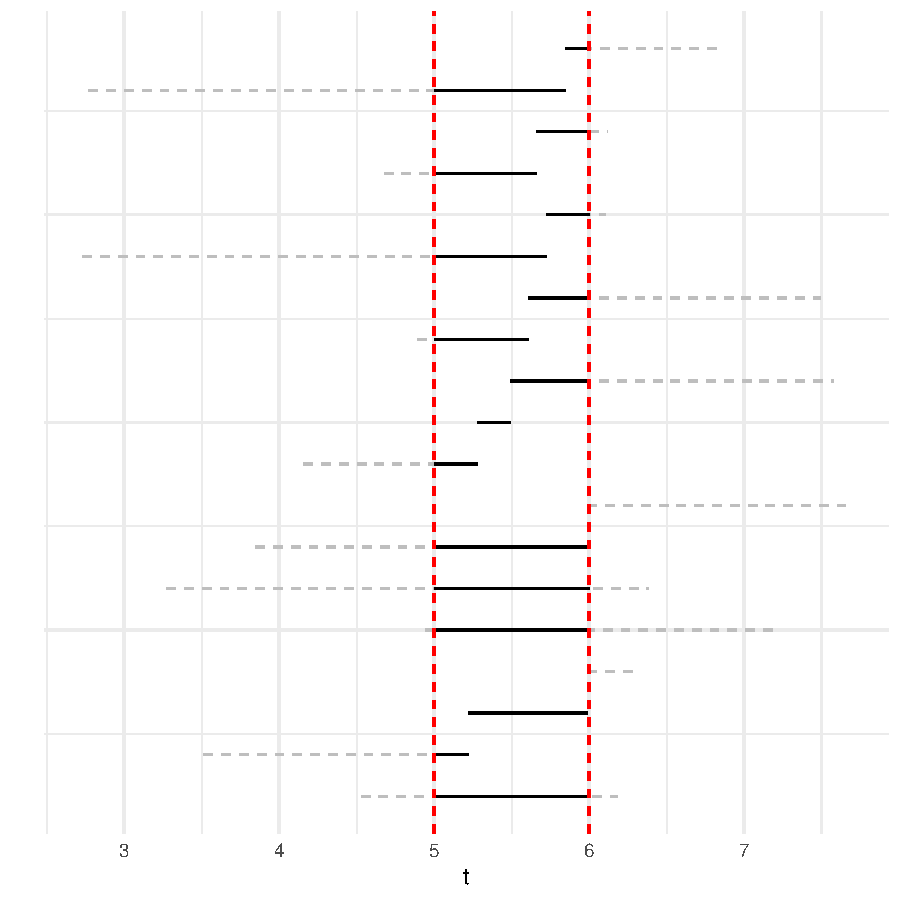
\includegraphics[width=1\textwidth]{./figures/ch-2/sim-data.pdf}
    \caption{The set of simulated lifetimes data. The exposure is shown on the horizontal axis, and the beginning and end of the observation period are shown as red vertical lines. The observed portions of the lifetimes are shown as solid black lines, while the unobserved portions are shown as dashed grey lines.}
    \label{fig:sim_censored_units}
\end{figure}

\begin{table}
\centering
\caption{\label{tab:sim-cmms-data}The simulated CMMS data for ten units.}
\centering
\begin{tabular}[t]{lrrrrr}
\toprule
Unit & Lifetime & True failure & True install & Observed install & Observed failure\\
\midrule
\cellcolor{gray!10}{1} & \cellcolor{gray!10}{1.66} & \cellcolor{gray!10}{6.18} & \cellcolor{gray!10}{4.53} & \cellcolor{gray!10}{5.00} & \cellcolor{gray!10}{6.00}\\
2 & 1.71 & 5.22 & 3.51 & 5.00 & 5.22\\
\cellcolor{gray!10}{2} & \cellcolor{gray!10}{0.77} & \cellcolor{gray!10}{5.99} & \cellcolor{gray!10}{5.22} & \cellcolor{gray!10}{5.22} & \cellcolor{gray!10}{5.99}\\
2 & 0.31 & 6.31 & 5.99 & 5.99 & 6.00\\
\cellcolor{gray!10}{3} & \cellcolor{gray!10}{2.28} & \cellcolor{gray!10}{7.23} & \cellcolor{gray!10}{4.94} & \cellcolor{gray!10}{5.00} & \cellcolor{gray!10}{6.00}\\
\addlinespace
4 & 3.11 & 6.38 & 3.27 & 5.00 & 6.00\\
\cellcolor{gray!10}{5} & \cellcolor{gray!10}{2.14} & \cellcolor{gray!10}{5.99} & \cellcolor{gray!10}{3.85} & \cellcolor{gray!10}{5.00} & \cellcolor{gray!10}{5.99}\\
5 & 1.69 & 7.68 & 5.99 & 5.99 & 6.00\\
\cellcolor{gray!10}{6} & \cellcolor{gray!10}{1.12} & \cellcolor{gray!10}{5.28} & \cellcolor{gray!10}{4.16} & \cellcolor{gray!10}{5.00} & \cellcolor{gray!10}{5.28}\\
6 & 0.21 & 5.50 & 5.28 & 5.28 & 5.50\\
\addlinespace
\cellcolor{gray!10}{6} & \cellcolor{gray!10}{2.08} & \cellcolor{gray!10}{7.58} & \cellcolor{gray!10}{5.50} & \cellcolor{gray!10}{5.50} & \cellcolor{gray!10}{6.00}\\
7 & 0.71 & 5.61 & 4.90 & 5.00 & 5.61\\
\cellcolor{gray!10}{7} & \cellcolor{gray!10}{1.89} & \cellcolor{gray!10}{7.50} & \cellcolor{gray!10}{5.61} & \cellcolor{gray!10}{5.61} & \cellcolor{gray!10}{6.00}\\
8 & 2.99 & 5.72 & 2.73 & 5.00 & 5.72\\
\cellcolor{gray!10}{8} & \cellcolor{gray!10}{0.39} & \cellcolor{gray!10}{6.11} & \cellcolor{gray!10}{5.72} & \cellcolor{gray!10}{5.72} & \cellcolor{gray!10}{6.00}\\
\addlinespace
9 & 0.98 & 5.66 & 4.68 & 5.00 & 5.66\\
\cellcolor{gray!10}{9} & \cellcolor{gray!10}{0.46} & \cellcolor{gray!10}{6.12} & \cellcolor{gray!10}{5.66} & \cellcolor{gray!10}{5.66} & \cellcolor{gray!10}{6.00}\\
10 & 3.07 & 5.85 & 2.77 & 5.00 & 5.85\\
\cellcolor{gray!10}{10} & \cellcolor{gray!10}{1.03} & \cellcolor{gray!10}{6.88} & \cellcolor{gray!10}{5.85} & \cellcolor{gray!10}{5.85} & \cellcolor{gray!10}{6.00}\\
\bottomrule
\end{tabular}
\end{table}


\subsection{Weakly informative prior} \label{subsec:weibull-model-fits}

I now fit the imputation model to the simulated data in Table~\ref{tab:sim-cmms-data} and compare the resulting posterior with the case where the installation times of the left-truncated samples are known and also with the alternative treatment of the unknown exposure histories, which is to discard all of the left-truncated samples. I fit these models with the weakly informative, independent Gaussian priors for $\beta$ and $\eta$ described in the right column of Table~\ref{tab:model-prior-comb} and previously mentioned in Sec.~\ref{sec:weibull-joint-prior}. The three Stan models are available on the GitHub repository. To sample from the posteriors, I use 4 chains, each 1000 iterations long with a burn-in of 500. Figure~\ref{fig:joint-post-weibull} shows the three posteriors. Plots (a), (b), and (c) in the figure show the joint draws of the two Weibull parameters for the fully observed, discarded, and imputed treatment of the left-truncated samples, respectively. The corresponding CDFs with uncertainty are shown in (d), (e), and (f). The true values of the parameters and the true CDF are plotted in red in the plots. The resulting inference from imputing the installation times of the left-truncated samples is almost the same as if we had fully observed the left-truncated samples. Discarding the left-truncated samples results in a much more diffuse posterior and, consequently, more uncertainty around the CDF, particularly for larger exposure times. Next, I refit the models using the version of the informative joint prior shown in Fig.~\ref{fig:kaminskiy-join-priors}~(c) and~(f), which informs the upper tail of the distribution.

\begin{figure}
    \centering
    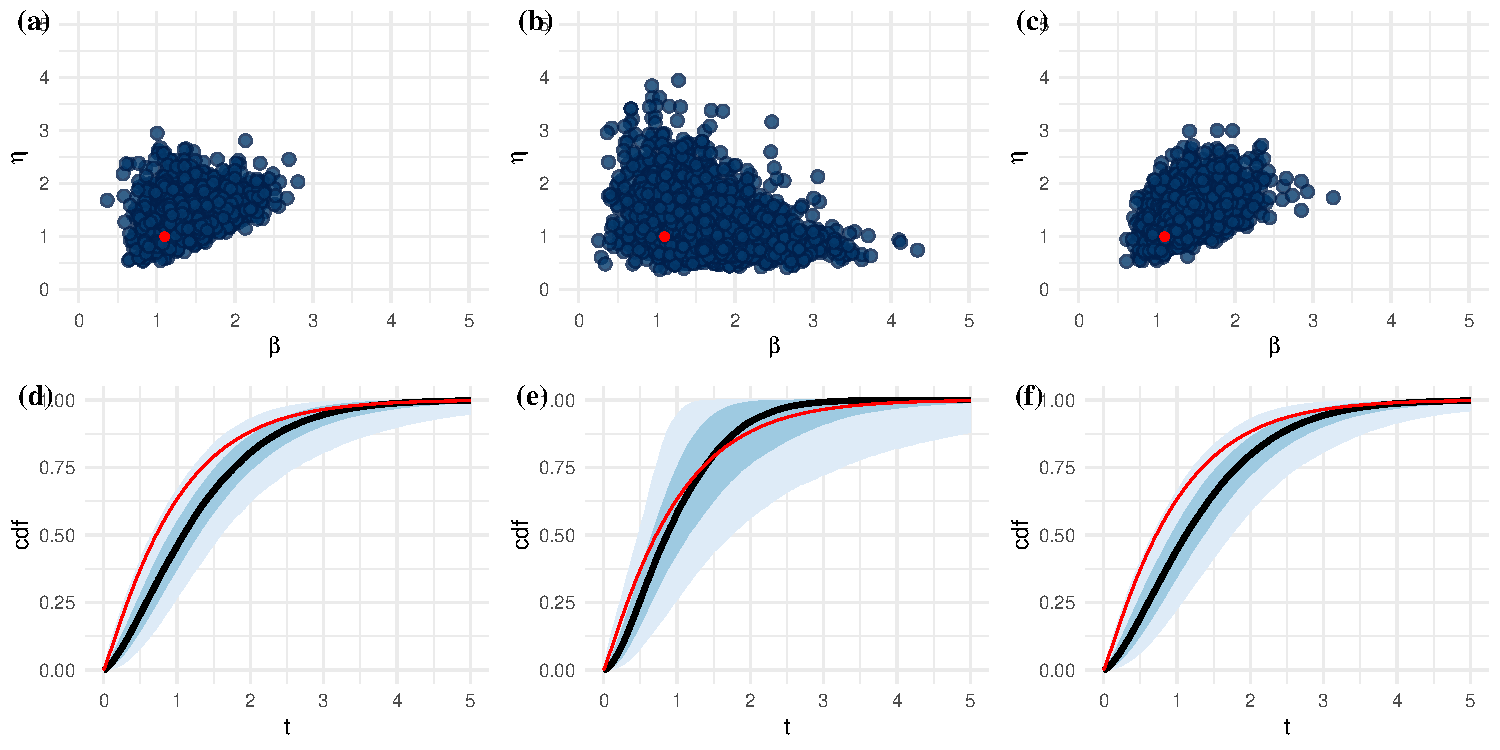
\includegraphics[width=1\textwidth]{./figures/ch-2/joint-posts.pdf}
    \caption{The draws from the joint posteriors conditioned on the simulated dataset when the left-truncated lifetimes are (a) fully observed, (b) discarded, or (c) imputed and a weakly informative prior is used. (d), (e), and (f) show the corresponding uncertainty around the CDF (in the form of the 0.5 and 0.8 uncertain intervals) that result from (a), (b), and (c), respectively. The true parameter values and CDF are shown in red.}
    \label{fig:joint-post-weibull}
\end{figure}

\subsection{Strongly informative prior} \label{subsec:weibull-model-fits-informative}

The prior in Fig.~\ref{fig:kaminskiy-join-priors}~(c) and~(f), which elicits information about the CDF at $t_1 = q_{0.80} = 1.54$ and $t_2 = q_{0.95} = 2.71$, strongly informs the Weibull model in the upper tail of the distribution but is sufficiently vague in the lower tail, where the data are strongly informative. Here, I refit the Weibull models with a slightly more diffuse version of the prior that increases the uncertainty around the estimates of the CDF at each elicitation time by using a larger value of the standard deviation. The informative joint prior is now
\begin{align*}
    \hat{F}_{t_1} \sim & \hbox{N}^{1}_{0}\left(0.8, 0.1\right)    \\
    \hat{F}_{t_2} \sim & \hbox{N}^{1}_{\hat{F}_{t_1}}\left(0.95, 0.05\right).
\end{align*}
Using the informative prior, I refit the three models from Sec.~\ref{subsec:weibull-model-fits}. Once again, I use 4 chains, each 1000 iterations long, with a burn-in of 500 to sample from the three posteriors. The resulting draws are plotted in (a), (b), and (c) of Fig.~\ref{fig:joint-post-weibull-inf} for the fully observed, discarded, and imputed treatment of the left-truncated samples, respectively. Comparing the posterior of the imputation method (plots~(c)) with the case where the left-truncated samples are fully observed (plots~(a)), the resulting inference is again very similar. However, using the informative prior, the posterior of the case where I have discarded the left-truncated samples, plot~(b), is much closer to the other two posteriors than when a vague prior is used. The corresponding posterior CDFs are shown in (d), (e), and (f) of Fig.~\ref{fig:joint-post-weibull-inf}. The uncertainty in all cases has been reduced, but most drastically in the upper right part of the CDF. In Fig.~\ref{fig:joint-post-weibull-inf}~(e), the effect of combining a likelihood that informs the CDF at lower exposure times with a prior that informs the CDF at higher exposure times has resulted in a more precise estimate of the CDF. 

\begin{figure}
    \centering
    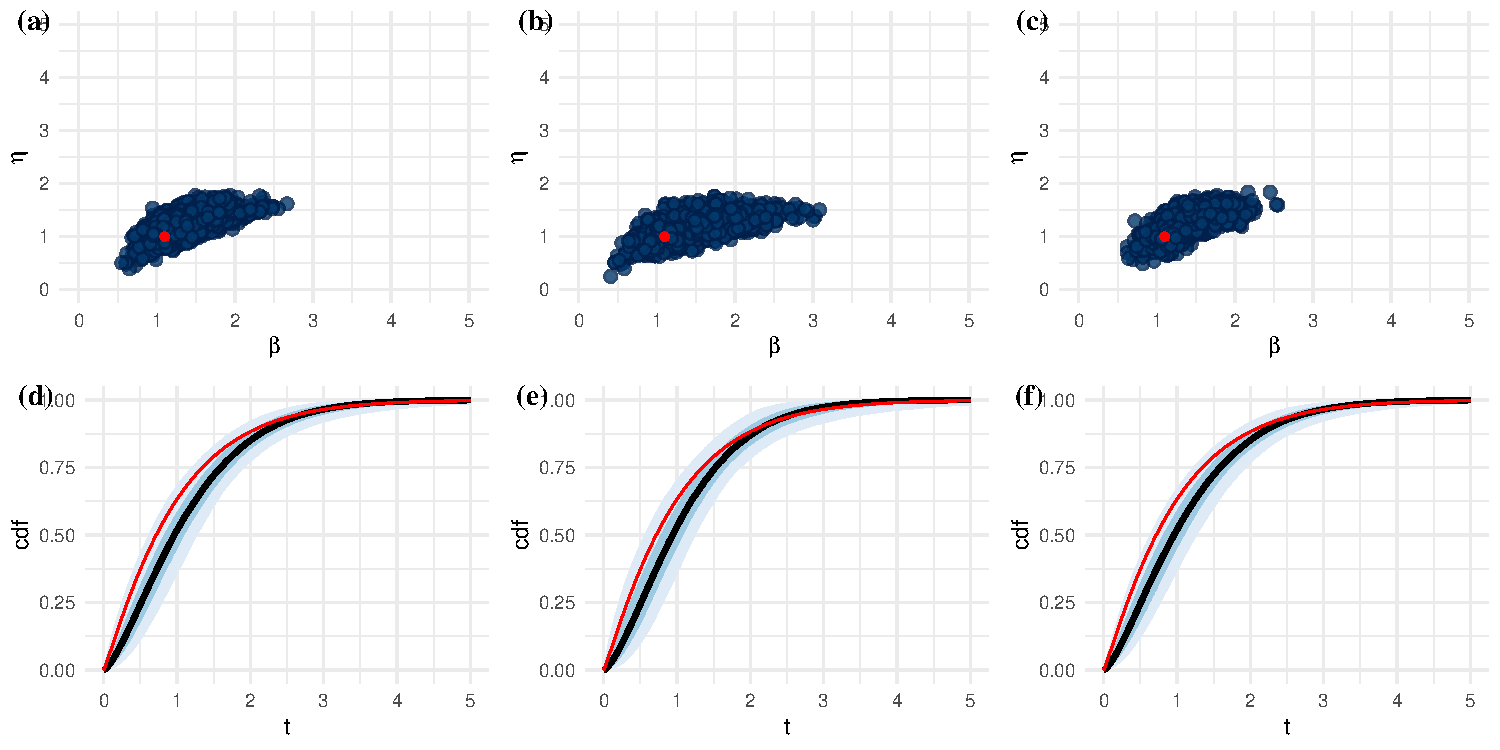
\includegraphics[width=1\textwidth]{./figures/ch-2/joint-posts-inf.pdf}
    \caption{The joint posteriors conditioned on the simulated dataset when the left-truncated lifetimes are (a) fully observed, (b) discarded, or (c) imputed and an informative joint prior is used that encodes information into the upper tail of the lifetime distribution. (d), (e), and (f) show the corresponding uncertainty around the CDF (in the form of the 0.5 and 0.8 uncertain intervals) that result from (a), (b), and (c), respectively. The true parameter values and CDF are shown in red.}
    \label{fig:joint-post-weibull-inf}
\end{figure}

In the implementation of the joint prior that I have used, the prior is properly updated through the MCMC routine, i.e, the observed data have updated our belief about the value of the CDF at both $t_1$ \emph{and} $t_2$. Figure~\ref{fig:weibull-prior-post-comp} compares the distribution of the posterior draws of $\hat{F}(t_i)$ (grey densities) with the prior (red curves). In the three plots in Fig.~\ref{fig:weibull-prior-post-comp}, the posterior distributions are clearly narrower than the prior, more so at $t_1$. Fitting the Weibull models to the data in Table~\ref{tab:sim-cmms-data} has shown that, for small sample sizes, in cases where we do not know the exposure history of the left-truncated samples the imputation method provides almost equivalent inference to the case where we had fully observed the left-truncated samples. Furthermore, discarding the left-truncated observations results in a large loss of information; however, this loss can be compensated for if there is prior information about longer lifetimes and this information is properly encoded into a joint prior. Here, I have shown one case for a small sample. Next, I devise a small simulation experiment to more rigorously evaluate the imputation method for the left-truncated samples with unknown exposure history.

\begin{figure}
    \centering
    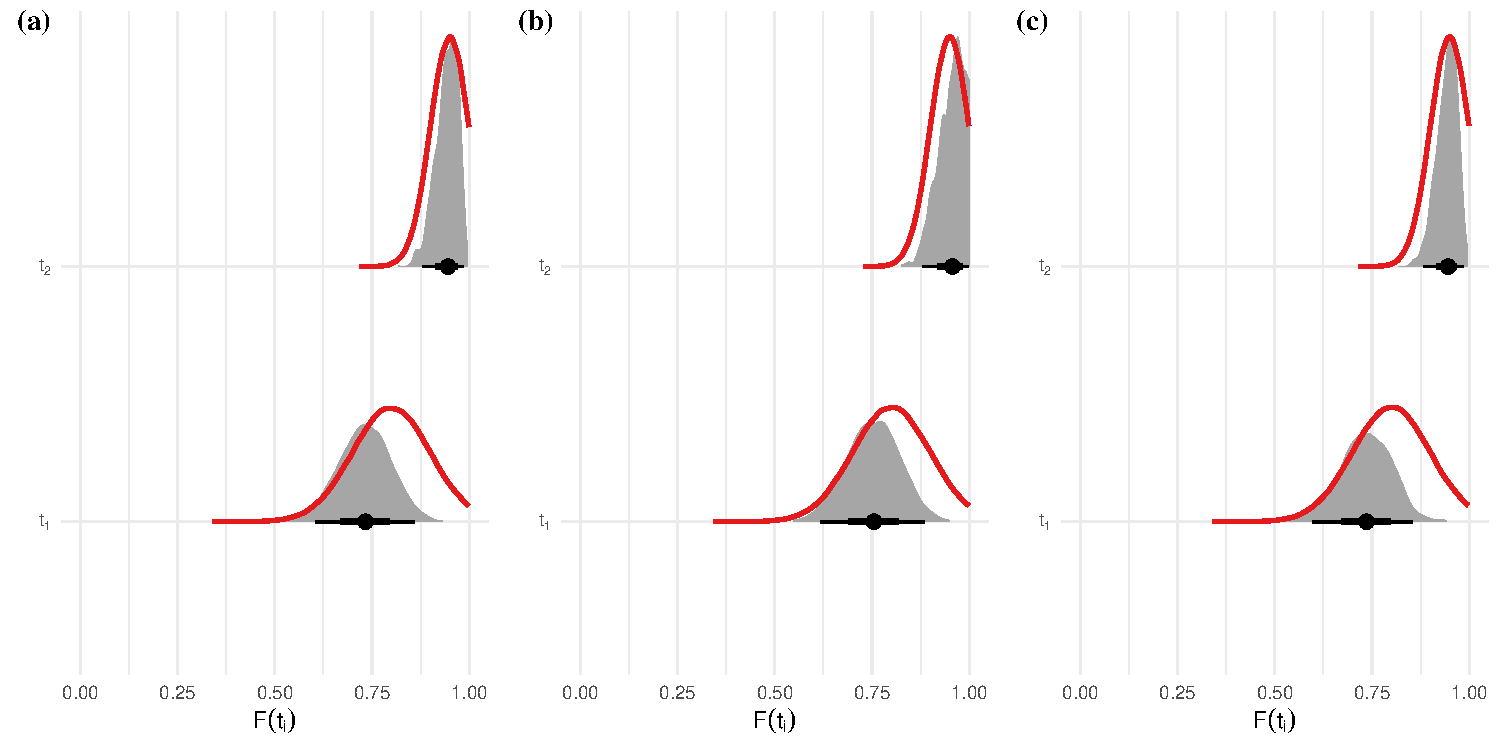
\includegraphics[width=0.8\textwidth]{./figures/ch-2/prior-post-comp.pdf}
    \caption{Comparison of the marginal prior and posterior for $F_{t_1}$ (top) and $F_{t_2}$ (bottom) when left-truncated lifetimes are (a) fully observed, (b) discarded, or (c) imputed to show how both the elicited distributions have been updated in the posterior.}
    \label{fig:weibull-prior-post-comp}
\end{figure}

\section{Simulation experiments} \label{sec:weibull-sim-study}

To explore the behaviour of the imputation method for left-truncated lifetimes with unknown exposure history, I repeat the simulation and model fitting process of Sec.~\ref{sec:weibull-sim-example} for several combinations of the simulation parameters: number of units, start of observation time, and length of observation time. Again I compare the imputation method (under both a vague and informative prior) with the alternative method of discarding the left-truncated observations as well as with the case where the left-truncated samples are fully observed (as ground truth). All of these comparisons are carried out using the same vague and informative priors used in Secs.~\ref{subsec:weibull-model-fits} and~\ref{subsec:weibull-model-fits-informative}. Section~\ref{subsec:factor-lvls} defines the factor levels of each simulation parameter that make up the factor combinations in the simulation experiments; Sec.~\ref{subsec:accuracy-measures} describes the measures of model accuracy that I use to compare the three models; and Sec.~\ref{subsec:sim-experiment-results} presents the results of the simulation experiments.

\subsection{Factor levels} \label{subsec:factor-lvls}

I vary three factors when simulating the datasets, each with three levels:
\begin{itemize}
    \item[] $N$: 10, 100, 500 units
    \item[] $t_{start}$: 1, 5, 15 mean lifetimes
    \item[] $(t_{end} - t_{start})$: 1, 3, 6 mean lifetimes.
\end{itemize}
In total, there are 27 factor combinations of the simulation parameters. Increasing the number of units, $N$, increases the sample size; increasing $t_{start}$ increases the range of possible values the left-truncated samples with unobserved truncation time can take (and therefore reduces the information they contribute); and increasing the window size, $t_{end} - t_{start}$, increases the number of fully observed lifetimes, the maximum length of the fully observed lifetimes and the number of samples that are both left-truncated and right-censored. For each factor combination, I perform 100 simulations, each time fitting the model and prior treatment as in Sec.~\ref{sec:weibull-sim-example} and described in Table~\ref{tab:model-prior-comb}. The flow of the simulation experiments is described in Alg.~\ref{algo:sim-experiments}. In total, there are $162 (=27 \times 6)$ factor-combinations and model-prior treatments each repeated one-hundred times.

\begin{algorithm}
	\caption{Structure of the simulation experiments.}
  \label{algo:sim-experiments}
	\begin{algorithmic}[1]
    \For {each factor combination of the simulation parameters, of with there are $(3\time3\times3) = 27$.}
    \State Simulate $100$ datasets using the simulation parameters.
    \State Fit each of the model-prior treatments---three model treatments and two prior treatments---to each of the datasets.
    \State Calculate the accuracy measures for each model fit.
    \EndFor
	\end{algorithmic} 
\end{algorithm} 

\subsection{Accuracy measures} \label{subsec:accuracy-measures}

To compare how well the Bayesian models recover the true data generating mechanism, I calculate the Bayesian $p$-values of the true parameter values, $\beta = 1.1$ and $\eta = 1$, from the fitted posteriors and the elppd of a dataset of 100 fully observed lifetimes generated from the true Weibull distribution. The Bayesian $p$-value for $\beta$ is easily calculated using the posterior draws as \citep{BDA2020}
\begin{equation*}
    \text{Pr}\left[\beta \ge \beta_{true}|y\right] = p_{\beta} = \frac{\sum^{S}_{s = 1}{\beta_{true} \le \beta_s}}{S},
\end{equation*}
where $\beta_{true}$ is the true value of $\beta$ used to simulate the data and $s = {1,\dots, S}$ are the draws from the posterior. The $p$-value of $\eta$ can be calculated using the same expression with $\eta$ in place of $\beta$. If the model posterior is well calibrated, then the $p$-values from repeating the same simulation should have a uniform distribution \citep{talts2020, stan_user_guide2024}\footnote{This manuscript and section \href{https://mc-stan.org/docs/stan-users-guide/simulation-based-calibration.html}{\textit{Simulation-Based Calibration}} from the Stan user guide discuss the concept of simulation-based calibration. What I do is not quite full simulation-based calibration, since I do not simulate the true values of the parameters from the prior, but many of the ideas should still hold.}. If the parameter estimates are unbiased, then the average $p$-values of the 100 repeated experiments for a factor combination will be near $0.5$. If the posterior uncertainty is overly diffuse, then the distribution of the 100 $p$-values will be concentrated around $0.5$, and if the uncertainty is too narrow, then the $p$-values will be pushed towards the boundaries (zero or one). The $p$-value provides an indication that the model posterior is well calibrated and if the parameter values are under or over-predicting, but does not express to what degree.

To determine the scale of any discrepancy, I also calculate the elppd of a new sample of 100 fully observed lifetimes under the different posteriors. I do this by simulating 100 datasets, each with 100 observations, and calculating the expected log-likelihood of each simulated dataset and then taking the average as follows:
\begin{equation*}
    \label{eq:elppd-100}
    \text{elppd}_{100} = \frac{\sum_{n = 1}^{100}\frac{1}{S}\sum_{s = 1}^{S}\sum_{i = 1}^{100}p(\tilde{y}_{n, i}|\beta_s, \eta_s)}{100}.
\end{equation*}

\subsection{Results} \label{subsec:sim-experiment-results}

Figures~\ref{fig:sim-study-pvalue} and~\ref{fig:sim-study-elppd} show the results of the simulation experiments. They show that under some circumstances, there is a slight bias in the posterior estimates of the parameters when the partially observed left-truncated lifetimes are imputed. There are two separate causes of the bias: the first comes from the mistreatment of lifetimes that are both left-truncated by the beginning of the observation period and right-censored by its end, and so only impacts inference when the observation period is short ($t_{end} - t_{start} = 1 \, \text{mean lifetime} = 0.95$); the second occurs because the uncertainty expressed in the posterior is an expression of \textit{our} uncertainty and therefore is not equivalent to frequentist confidence intervals, and so the $p$-values appear biased. The scale of this second source of bias is smaller. Despite these two sources of bias, elppd results suggest that in some cases, it is better to use the slightly biased treatment in favour of discarding the left-truncated lifetimes because the precision of the posterior places more mass around the true data-generating mechanism, particularly if a weak prior is used.

Figure~\ref{fig:sim-study-pvalue} summarises the $p$-values of the 100 simulation runs under each factor combination by their means. The different treatments of the left-truncated lifetimes---fully observed, imputed, or discarded---are shown as different colours and the type of prior---informative or vague---is shown as different point types. For example, fully observed left-truncated lifetimes and a strongly informative prior is shown as a blue dot. If the model's posterior is unbiased, then the point should sit in the centre of each plot, i.e., an average $p$-value of $0.5$ for both parameters. If the average of the p-vales is at one or zero, then there is typically very little posterior mass around the true parameter value, and hence, we can conclude that the inference is biased. When $N = 10$, the bias in parameter estimates is negligible compared to the uncertainty in the posterior, so all of the different treatment-prior combinations perform similarly. However, as the number of units increases and the sample size gets larger, the posteriors become more precise, and the bias becomes more obvious.

\begin{figure}
    \centering
    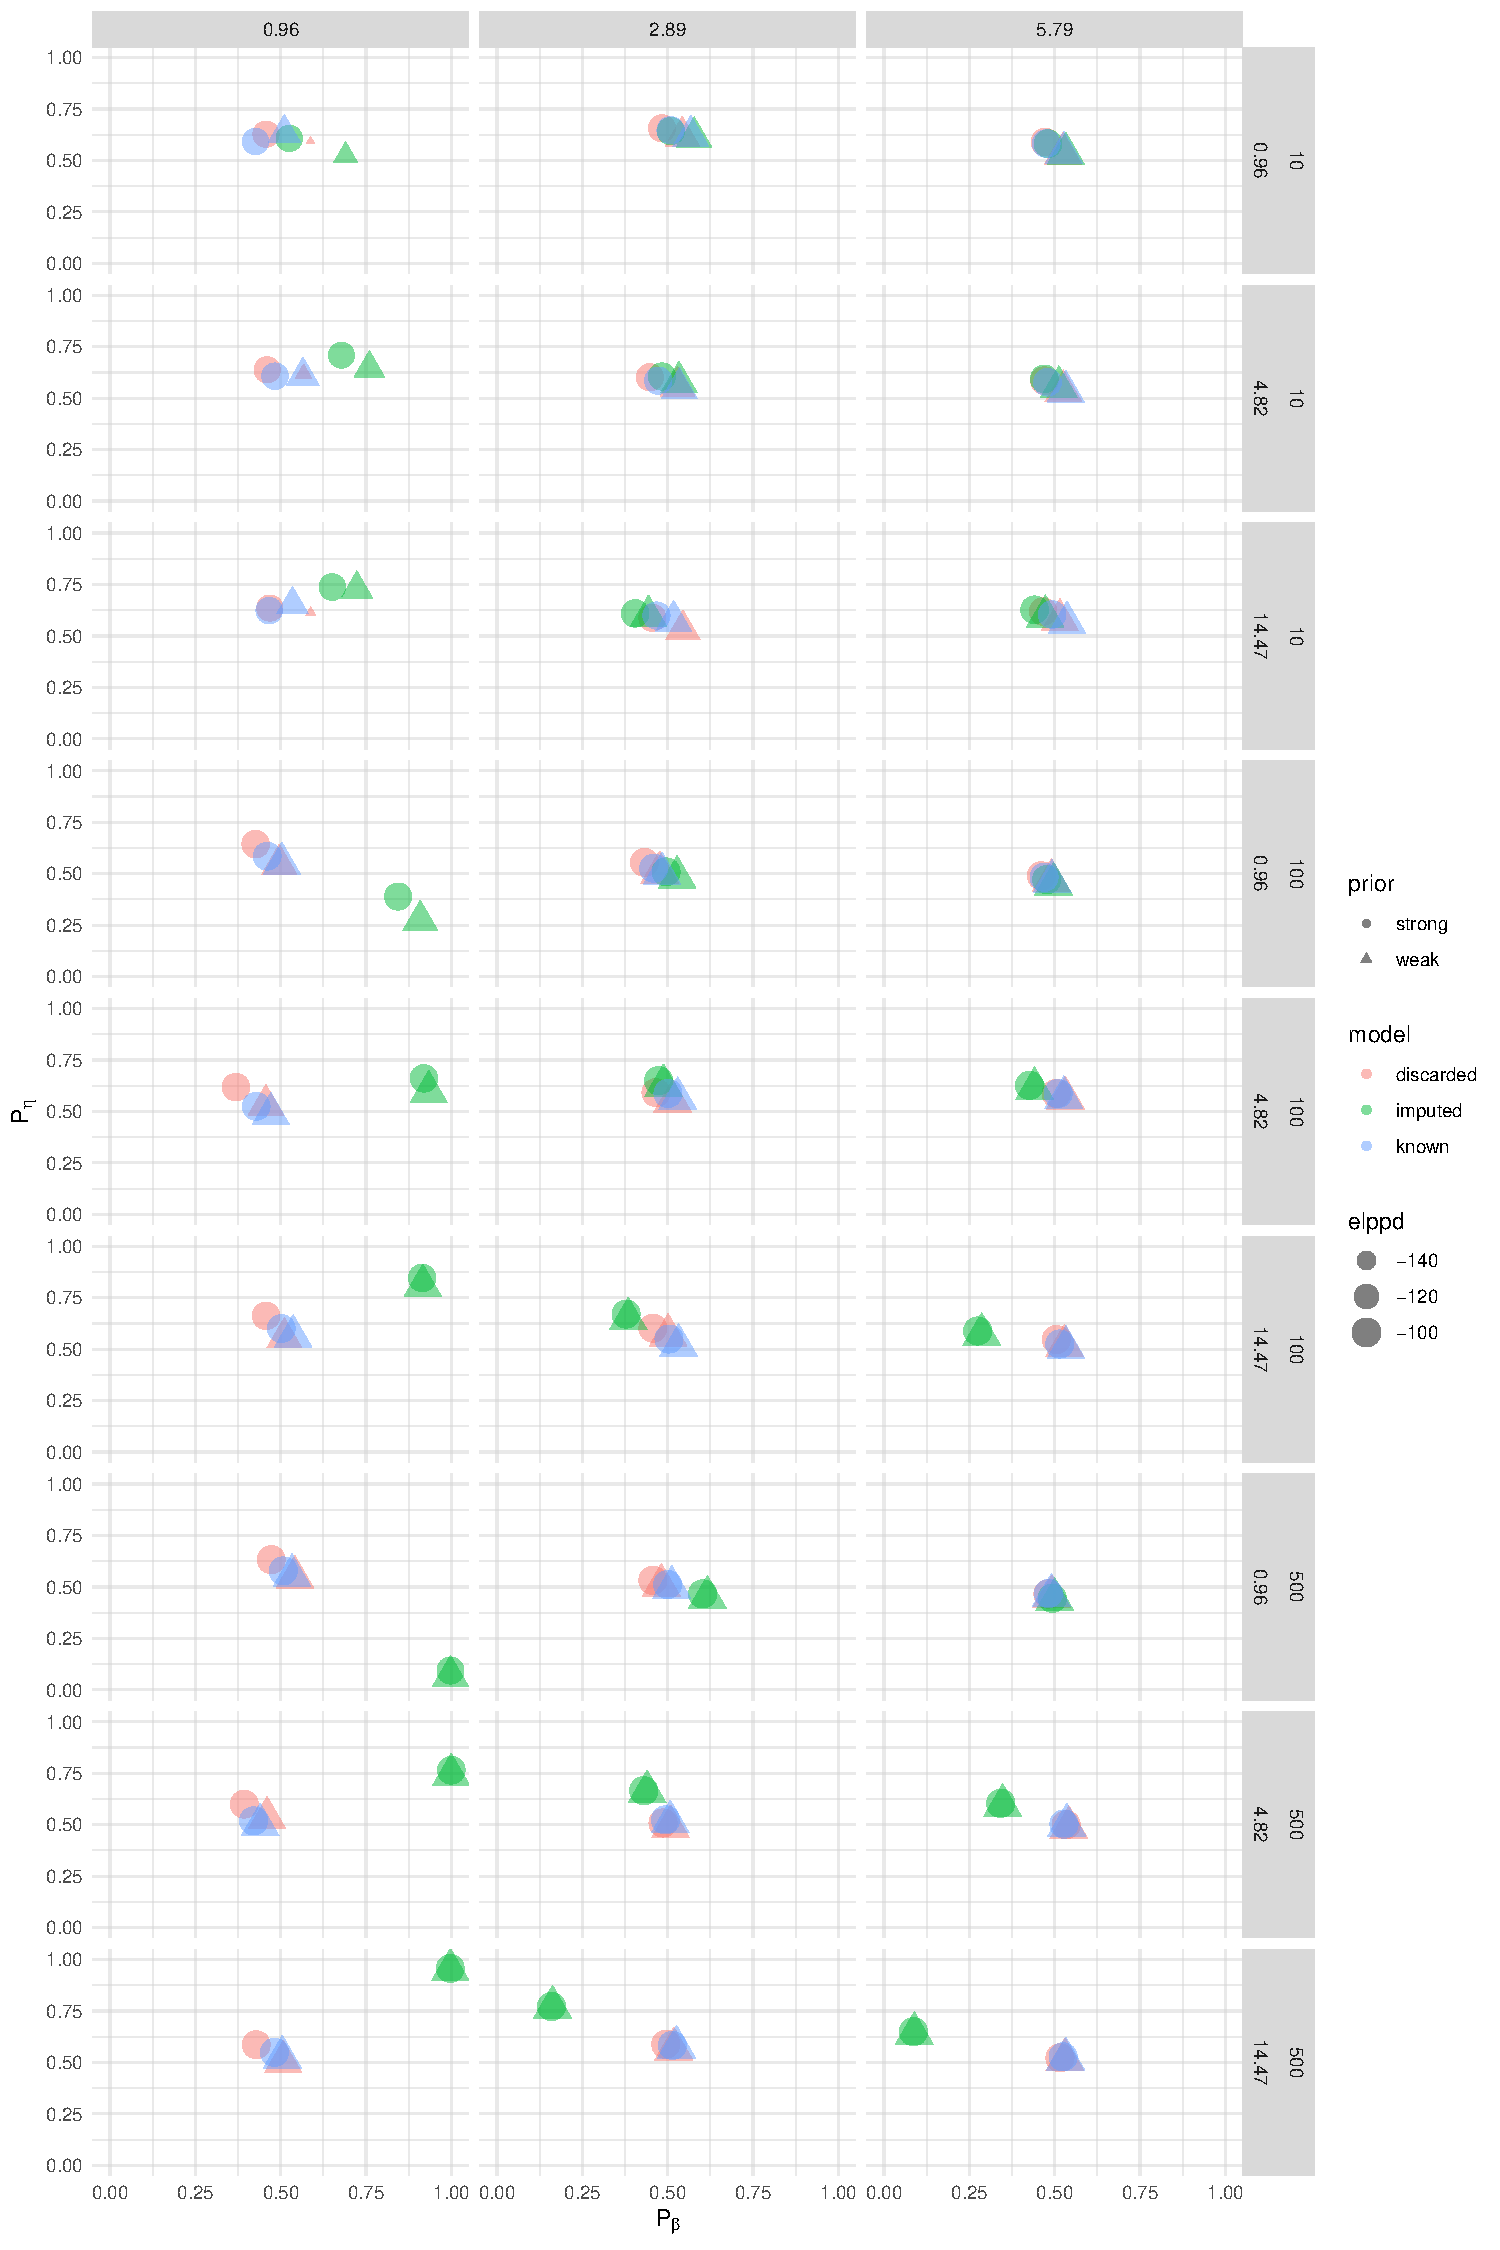
\includegraphics[width=0.8\textwidth]{./figures/ch-2/sim-results-pvalues.pdf}
    \caption{The simulation results are summarised by the mean of the 100 repetitions for each factor combination. The columns show the three levels of $t_{end} - t_{start}$, and the rows show the levels of $t_{start}$ and $N$. The Bayesian $p$-values of $\beta$ and $\eta$ are reported on the horizontal and vertical axis, respectively, and the colours of the points show the treatment of the left-truncated samples, and the shape shows the prior. The size of the points correspond the the average $\text{elppd}_{100}$ calculated according to eq.~\eqref{eq:elppd-100}}.
    \label{fig:sim-study-pvalue}
\end{figure}

The leftmost column in Fig.~\ref{fig:sim-study-pvalue} shows the simulations where the window size is equal to one mean lifetime, $t_{end} - t_{start} = 0.95$. In this case, there is a high proportion of lifetimes that begin before the start of the observation period and end after the observation period: they are both left-truncated at the beginning and right-censored at the end. For these cases, the Bayesian $p$-value of the shape parameter, $\beta$, is greater than $0.5$ and, depending on the value of $t_{start}$, the scale parameter $\eta$ is either over ($p_{\eta} > 0.5$) or under ($p_{\eta} < 0.5$) estimated. Bias when $t_{start}$ is small is expected since the assumption of uniform entry I make in the model in eq.~\eqref{eq:imp-trun-times} is not valid since there is a higher chance that lifetimes were installed at $t_0$. However, the bias in the cases where $t_{start} << 0$ is unexpected. Inspecting the posteriors more closely shows that the HMC algorithm is updating the random variable $\tau^L$ in eq.~\eqref{eq:imp-trun-times}, where it should instead be treated as a nuisance parameter and excluded from the updating procedure. This occurs because of the way the HMC algorithm in Stan is implemented: it is not possible to cut the flow of information\footnote{The Stan user forum has some commentary on the matter by Bob Carpenter \href{https://discourse.mc-stan.org/t/generating-random-numbers-in-the-model/3608/2}{here}.}. For the cases where $t_{end} - t_{start} > 1$ mean lifetime, the proportion of lifetimes that are both left-truncated and right-censored is low, and hence, so is the bias that results from the treatment of these observations. 

In Fig.~\ref{fig:sim-study-pvalue}, when $t_{end} - t_{start} > 1$ (the two right-most columns), the posterior where the left-truncated lifetimes are imputed is more similar to the posterior from the other two treatments. However, as the number of units is increased, a slight underestimation of the shape parameter $\beta$ becomes apparent when $t_{start} >> 0$. However, even for the factor combinations where $N = 500$ and $t_{end} - t_{start} = 6$ mean lifetimes---the combination that results in the largest sample size and hence the narrowest posterior---the average $p$-value of $\beta$ is still not zero, showing that even when the posterior is extremely precise it still generally contains the true parameter value. This second apparent bias is more a result of the uncertainty that we have encoded into the model, which does not align with the frequentist interpretation of uncertainty intervals that $p$-values measure. When $t_{start}$ is large, the upper bound of the partially observed left-truncated lifetimes is increased. Extending the support of these random variables means that the upper tails become heavier, and so too does the posterior of the Weibull shape parameter. This second form of bias is only noticeable when the number of units is very large ($N = 500$), and so, in most cases, it would be unnoticeable over the uncertainty in the posterior.

Despite both sources of bias, the elppd of 100 new observations generated from the true Weibull model is very close for all treatment-prior combinations. In Fig.~\ref{fig:sim-study-pvalue}, the size of the points indicates the average values of $\text{elppd}_{100}$ calculated according to eq.~\eqref{ep:computed_elppd}. From this we can see that the only noticeable difference between the three treatments of the left-truncated data is that when there is a short period of observation ($t_{end} - t_{start} = 0.95$) and there are few units ($N = 10$) discarding the left-truncated observations has a large impact on the elppd if the analysis is not supplemented by an informative joint prior. This has already been shown in Fig.~\ref{fig:joint-post-weibull}~(b) and~(e). Figure~\ref{fig:sim-study-elppd} compares the average $\text{elppd}_{100}$ scores under the different factor combinations more closely. In the figure, columns show the different levels of $t_{end} - t_{start}$ and rows show the different levels of $t_{start}$; the levels of $N$ are plotted on the horizontal axis, and the treatment of the left-truncated samples and the type of prior are shown by the colour and shape of the point respectively. The plotted elppd values show that when there are few units or a short period of observation, the method of imputing the partially observed values of the left-truncated samples results in an $\text{elppd}_{100}$ score that is closer to the fully observed treatment than if we were to discard the partially observed left-truncated lifetimes, except when $t_{start} = 1$ mean lifetime. The fact that it is hard to distinguish between the approaches based on the $\text{elppd}_{100}$ score, despite the bias, shows that the scale of the bias is typically inconsequential.

\begin{figure}
    \centering
    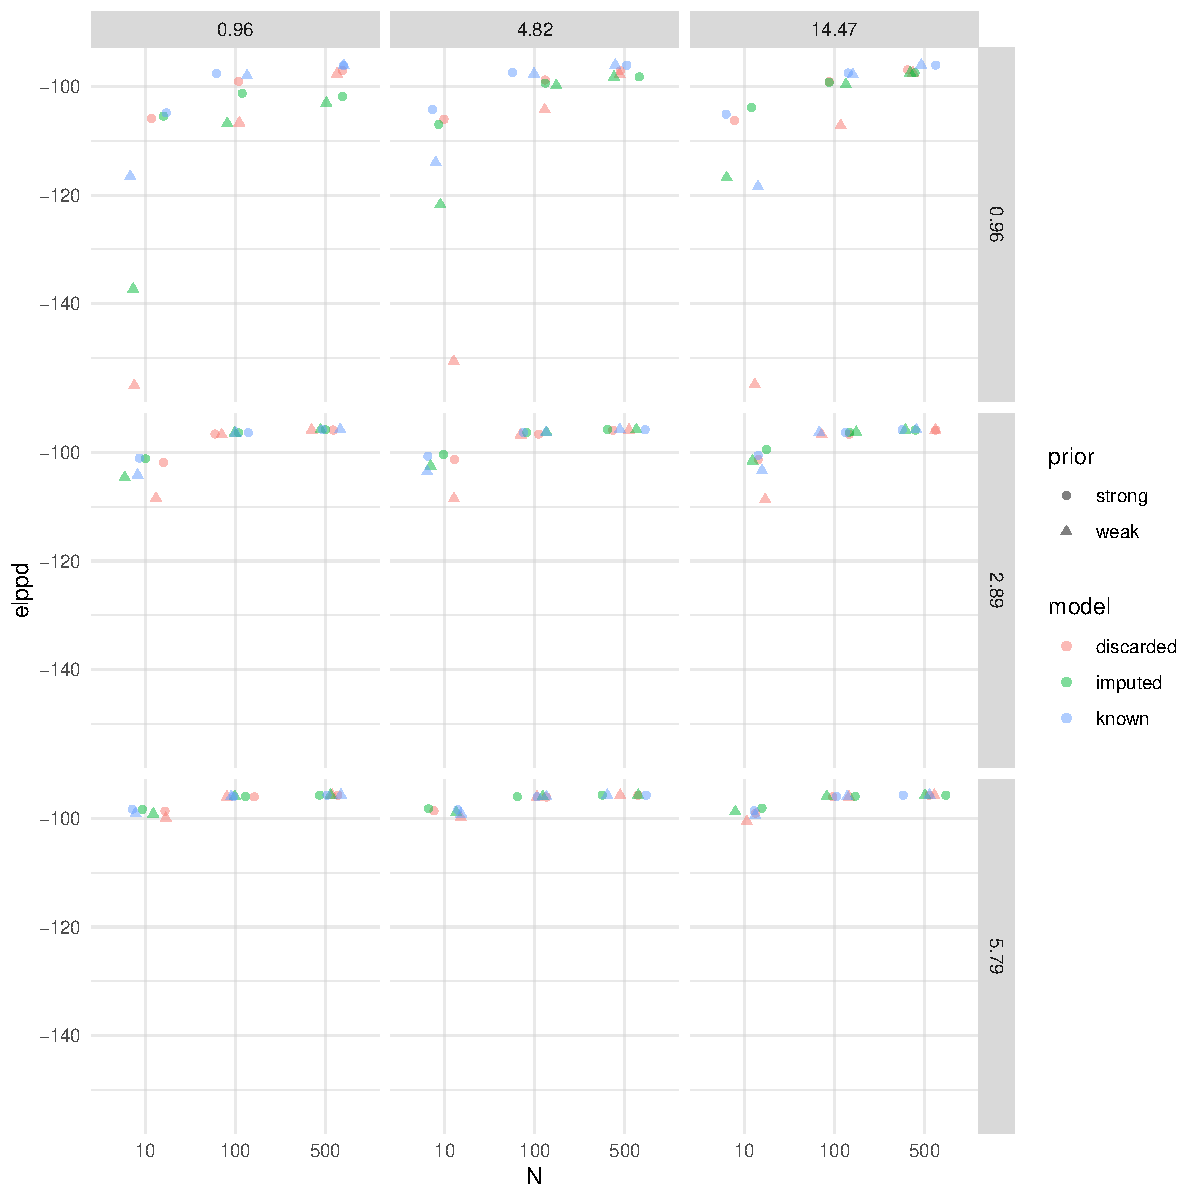
\includegraphics[width=0.8\textwidth]{./figures/ch-2/sim-results-elppd.pdf}
    \caption{The $\text{elppd}_{100}$ simulation results summarised by the mean of the 100 repetitions for each factor combination. The columns show the different levels of $t_{end} - t_{start}$ and rows the different levels of $t_{start}$. The number of units $N$ is shown on the horizontal axis, and the average $\text{elppd}_{100}$ score is shown on the vertical axis. The colours of the points show the treatment of the left-truncated samples and the shape shows the prior.}
    \label{fig:sim-study-elppd}
\end{figure}

\section{Concluding remarks} \label{sec:weibull-conclusion}

In this chapter, I have shown that when censored observations are treated as missing and their values imputed instead of being integrated out, observations that are left-truncated with unknown exposure history can be treated as a case of interval-censoring, and as a result, their partially observed value and truncation time imputed through Bayesian analysis. Doing so retains the information in the left-truncated samples, resulting in much more precise estimates than the alternative option, which is simply to discard the left-truncated lifetimes. I also extend on the method proposed by \citet{kaminskiy2005} for constructing a joint prior for the Weibull parameters by demonstrating how the choice of the two elicitation times, $t_1$ and $t_2$, dictates where in the lifetime distribution information is encoded, i.e., in the lower or upper tail, and implement the prior in a fully Bayesian model for left-truncated and right-censored lifetime data. The latter ensures the joint draws from the informative prior are properly filtered through the likelihood, and hence our prior belief around the CDF at both $t_1$ and $t_2$ is updated in the posterior.

I used a simulation example to demonstrate the method to impute left-truncated lifetimes with unknown exposure history and their corresponding truncation times alongside the alternative case where the left-truncated samples are discarded and the case where the left-truncated samples are fully observed. I fitted all three cases with both a vague and informative joint prior. When a vague prior is used, imputing the left-truncated lifetimes with unknown exposure history retains the extra information in these samples, resulting in a much more precise posterior than when the left-truncated samples are discarded, and roughly the same inference as when the lifetimes are fully observed. When a carefully constructed joint prior is used, which encodes information in the upper tail of the lifetime distribution, the posterior where the left-truncated samples have been discarded is much closer to the other two posteriors---where the left-truncated lifetimes are fully observed or imputed.

Finally, I performed a small simulation experiment to explore the two approaches of imputing or discarding the left-truncated samples with unknown exposure times---with and without an informative prior---under different simulation scenarios. The simulation experiments show that imputing the left-truncated lifetimes and truncation times results in a slight bias in the parameter estimates, but in most cases this bias is small relative to the uncertainty in the posterior. There are two sources of bias. The first comes about because of the treatment of observations that are both left-truncated/interval-censored by the start of the observation period and right-censored by its end. For these lifetimes, I make the assumption that the entry time is uniformly distributed by assigning a uniform prior to the parameter $\tau^L$. However, this parameter is included in the updating procedure of the HMC algorithm. To remove the bias, the model should be re-implemented either in an alternative probabilistic programming language such as BUGs, where nuisance parameters that are not updated can be included in the MCMC procedure, or using a custom MCMC algorithm for the model. However, this is only needed if the observation period is small enough to result in a large proportion of lifetimes that are left-truncated and right-censored.

The second source of bias arises because imputing the left-truncated lifetimes and their truncation times results in uncertainty intervals that are not equivalent to frequentist confidence intervals but rather encode \textit{our} uncertainty. This bias is small, and the true value of the parameters is still contained in the posterior. However, in all cases, the elppd of a new set of 100 fully observed lifetimes from the true data-generating mechanism are very close, showing that the scale of the bias is relatively negligible.

\paragraph*{Recommendations}
Based on the learnings from this chapter, it should be suitable to use the proposed approach for data that are left-truncated with unknown installation times, so long as the observation period is sufficiently long. However, suppose there is a strong likelihood based on sample size, and the analyst requires a very accurate estimation of the parameter values. In such a case, it is better to discard partially observed left-truncated lifetimes and, if information is available to do so, construct an informative joint prior that informs the upper tail of the distribution. Otherwise, when the likelihood is weaker, using the imputation method results in a posterior that is almost equivalent to the case where the installation times of the left-truncated lifetimes are known and the posterior uncertainty still contains the true model.

In the next chapter, I use the methods proposed here and the learnings of the simulation experiments to analyse the idler-frame dataset and show that when lifetime analysis is performed in the Bayesian framework and the censored observations are imputed, MCMC sampling naturally provides estimates and uncertainty intervals for the failure times of units still in operation, the expected number of failures in the next short time interval, and the cost per unit time of a preventative replacement strategy.